%%%%%%%%%%%%%%%%%%%%%%%%%%%%%%%%%%%%%%%%%
% The Legrand Orange Book
% LaTeX Template
% Version 1.3 (21/8/13)
%
% This template has been downloaded from:
% http://www.LaTeXTemplates.com
%
% Original author:
% Mathias Legrand (legrand.mathias@gmail.com)
%
% License:
% CC BY-NC-SA 3.0 (http://creativecommons.org/licenses/by-nc-sa/3.0/)
%
% Compiling this template:
% This template uses biber for its bibliography and makeindex for its index.
% When you first open the template, compile it from the command line with the 
% commands below to make sure your LaTeX distribution is configured correctly:
%
% 1) pdflatex main
% 2) makeindex main.idx -s StyleInd.ist
% 3) biber main
% 4) pdflatex main x 2
%
% After this, when you wish to update the bibliography/index use the appropriate
% command above and make sure to compile with pdflatex several times 
% afterwards to propagate your changes to the document.
%
% This template also uses a number of packages which may need to be
% updated to the newest versions for the template to compile. It is strongly
% recommended you update your LaTeX distribution if you have any
% compilation errors.
%
% Important note:
% Chapter heading images should have a 2:1 width:height ratio,
% e.g. 920px width and 460px height.
%
%%%%%%%%%%%%%%%%%%%%%%%%%%%%%%%%%%%%%%%%%

%----------------------------------------------------------------------------------------
%	PACKAGES AND OTHER DOCUMENT CONFIGURATIONS
%----------------------------------------------------------------------------------------

\documentclass[11pt,fleqn]{book} % Default font size and left-justified equations 
\usepackage{logreq}
\usepackage{pdflscape}
\usepackage{ifthen}
\newboolean{tablet}
\newboolean{fullBook}
\newboolean{includeCover}
% Change the boolean below from true to false to disactivate tablet output.
\setboolean{tablet}{true} 
\setboolean{fullBook}{true}
\setboolean{includeCover}{true}
\newcommand{\ignore}[1]{ %ignored
}
%\usepackage[top=3cm,bottom=3cm,left=3.2cm,right=3.2cm,headsep=10pt,a4paper]{geometry} % Page margins
%
% define \iftablet and set its value:
\ifthenelse {\boolean{tablet}}{
% for tablets:
\usepackage[papersize={5in,6in},margin=3mm]{geometry} 

} {
\usepackage[top=3cm,bottom=2.5cm,left=3.5cm,right=3.5cm,headsep=10pt,paperwidth=8.25in, paperheight=10.25in, hmarginratio=2:3]{geometry} % Page margins
%Turn on to enable Bleed and Trim boxes
\pdfpageattr{
/MediaBox [0	0	594	738] 
/BleedBox [9	9	585	729]
/CropBox  [0	0	594	738]
/TrimBox  [9	9	585	729]
}
}
% Try to expand space between figure number and caption in listoffigures

%\usepackage{tocstyle} 
%\usetocstyle{standard}

\usepackage{xcolor} % Required for specifying colors by name
\definecolor{ocre}{RGB}{243,102,25} % Define the orange color used for highlighting throughout the book

% Font Settings
\usepackage{avant} % Use the Avantgarde font for headings
%\usepackage{times} % Use the Times font for headings
\usepackage{mathptmx} % Use the Adobe Times Roman as the default text font together with math symbols from the Sym­bol, Chancery and Com­puter Modern fonts

\usepackage{microtype} % Slightly tweak font spacing for aesthetics
\usepackage[utf8]{inputenc} % Required for including letters with accents
\usepackage[T1]{fontenc} % Use 8-bit encoding that has 256 glyphs

% Use typewriter font that supports bold:
\usepackage[scaled]{beramono}

% Bibliography
\usepackage[style=alphabetic,sorting=nyt,sortcites=true,autopunct=true,babel=hyphen,hyperref=true,abbreviate=false,backref=true,backend=biber]{biblatex}
\addbibresource{bibliography.bib} % BibTeX bibliography file
\defbibheading{bibempty}{}

% Index
\usepackage{calc} % For simpler calculation - used for spacing the index letter headings correctly
\usepackage{makeidx} % Required to make an index
\makeindex % Tells LaTeX to create the files required for indexing

% Load side caption. See http://tex.stackexchange.com/questions/49979/put-text-to-the-right-of-figures
\usepackage[innercaption]{sidecap}
\sidecaptionvpos{figure}{t}

%\usepackage{listings}
\usepackage{fancyvrb}

\usepackage{color}

\definecolor{dkgreen}{rgb}{0,0.6,0}
\definecolor{gray}{rgb}{0.5,0.5,0.5}
\definecolor{mauve}{rgb}{0.58,0,0.82}
\definecolor{lightblue}{rgb}{0.54,0.824,1}

\usepackage{mathtools}
\usepackage{stmaryrd}
%----------------------------------------------------------------------------------------
%\usepackage{layout}

\ifthenelse {\boolean{tablet}}{
\setboolean{includeCover}{false}
\newcommand{\coverScalingFactor}[0]{0.63}
\newcommand{\miniTocHeight}[0]{5cm}
\newcommand{\roundChapterTitleXOffset}[0]{5cm}
\newcommand{\roundChapterTitleYOffset}[0]{4cm}
\newcommand{\NewChapterTextOffsetY}[0]{130\p@}
\newcommand{\ChapterFontStyle}[0]{\Large}
\newcommand{\sectionMarginPosition}[0]{-\textwidth}
\newcommand{\widthProjectTabFigure}[0]{5cm}
\newcommand{\XHeadingOffset}[0]{1cm}
\newcommand{\YHeadingOffset}[0]{0.25cm}
}{
\newcommand{\coverScalingFactor}[0]{1.04}
\newcommand{\miniTocHeight}[0]{6cm}
\newcommand{\roundChapterTitleXOffset}[0]{8.5cm}
\newcommand{\roundChapterTitleYOffset}[0]{6.5cm}
\newcommand{\NewChapterTextOffsetY}[0]{180\p@}
\newcommand{\ChapterFontStyle}[0]{\huge}
\newcommand{\sectionMarginPosition}[0]{1em}
\newcommand{\widthProjectTabFigure}[0]{7cm}
\newcommand{\XHeadingOffset}[0]{0.8in}
\newcommand{\YHeadingOffset}[0]{-0.5cm}
}

\newcommand{\mytilde}{\raise.17ex\hbox{$\scriptstyle\mathtt{\sim}$}}

% When the first line is active, we print the questions to Jetbrains and mark the location in the index.
%\newcommand{\questionToJetBrains}[1]{Q: #1\index{Question to Jetbrains}}
\newcommand{\questionToJetBrains}[1]{}


%----------------------------------------------------------------------------------------
%	VARIOUS REQUIRED PACKAGES
%----------------------------------------------------------------------------------------

\usepackage{titlesec} % Allows customization of titles

\usepackage{graphicx} % Required for including pictures
\graphicspath{{Pictures/}} % Specifies the directory where pictures are stored


\usepackage{lipsum} % Inserts dummy text

\usepackage{paralist}
\usepackage{tikz} % Required for drawing custom shapes

\usepackage[english]{babel} % English language/hyphenation

\usepackage{enumitem} % Customize lists
\setlist{nolistsep} % Reduce spacing between bullet points and numbered lists

\usepackage{booktabs} % Required for nicer horizontal rules in tables

\usepackage{eso-pic} % Required for specifying an image background in the title page

% To Get keys like \return \cmdkey \keys{} \menu{}
\usepackage{menukeys}

% To get the \BibTex command:
\usepackage{dtklogos}

\usepackage{stringstrings}

%----------------------------------------------------------------------------------------
%	MAIN TABLE OF CONTENTS
%----------------------------------------------------------------------------------------

\usepackage{titletoc} % Required for manipulating the table of contents

% 
%  Configure sections and subsections for tablet format:
%
\ifthenelse {\boolean{tablet}}{
% for tablets:
\newcommand{\positionSection}[0]{1.25cm}
}{
}
% Chapter text styling
\titlecontents{chapter}[1.25cm] % Indentation
{\addvspace{15pt}\large\sffamily\bfseries} % Spacing and font options for chapters
{\color{ocre!60}\contentslabel[\Large\thecontentslabel]{1.25cm}\color{ocre}} % Chapter number
{}  
{\color{ocre!60}\normalsize\sffamily\bfseries\;\titlerule*[.5pc]{.}\;\thecontentspage} % Page number
% Section text styling
\titlecontents{section}[1.25cm] % Indentation
{\addvspace{5pt}\sffamily\bfseries} % Spacing and font options for sections
{\contentslabel[\thecontentslabel]{1.25cm}} % Section number
{}
{\sffamily\hfill\color{black}\thecontentspage} % Page number
[]
% Subsection text styling
\titlecontents{subsection}[1.25cm] % Indentation
{\addvspace{1pt}\sffamily\small} % Spacing and font options for subsections
{\contentslabel[\thecontentslabel]{1.25cm}} % Subsection number
{}
{\sffamily\;\titlerule*[.5pc]{.}\;\thecontentspage} % Page number
[] 


% Figure LOF text styling
\titlecontents{figure}[1.25cm] % Indentation
{\addvspace{5pt}\sffamily} % Spacing and font options for chapters
{\contentslabel[\thecontentslabel]{1.25cm}} % Chapter number
{}  
{\normalsize\sffamily\;\titlerule*[.5pc]{.}\;\thecontentspage} % Page number


%----------------------------------------------------------------------------------------
%	MINI TABLE OF CONTENTS IN CHAPTER HEADS
%----------------------------------------------------------------------------------------

% Section text styling
\titlecontents{lsection}[0em] % Indenting
{\footnotesize\sffamily} % Font settings
{}
{}
{}

% Subsection text styling
\titlecontents{lsubsection}[.5em] % Indentation
{\normalfont\footnotesize\sffamily} % Font settings
{}
{}
{}
 
%----------------------------------------------------------------------------------------
%	PAGE HEADERS
%----------------------------------------------------------------------------------------

\usepackage{fancyhdr} % Required for header and footer configuration

\pagestyle{fancy}
\renewcommand{\chaptermark}[1]{\markboth{\sffamily\normalsize\bfseries #1}{}} % Chapter text font settings
\renewcommand{\sectionmark}[1]{\markright{\sffamily\normalsize\thesection\hspace{5pt}#1}{}} % Section text font settings
\fancyhf{} \fancyhead[LE,RO]{\sffamily\normalsize\thepage} % Font setting for the page number in the header
\fancyhead[LO]{\rightmark} % Print the nearest section name on the left side of odd pages
\fancyhead[RE]{\leftmark} % Print the current chapter name on the right side of even pages
\renewcommand{\headrulewidth}{0.5pt} % Width of the rule under the header
\addtolength{\headheight}{2.5pt} % Increase the spacing around the header slightly
\renewcommand{\footrulewidth}{0pt} % Removes the rule in the footer
\fancypagestyle{plain}{\fancyhead{}\renewcommand{\headrulewidth}{0pt}} % Style for when a plain pagestyle is specified

% Removes the header from odd empty pages at the end of chapters
\makeatletter
\renewcommand{\cleardoublepage}{
\clearpage\ifodd\c@page\else
\hbox{}
\vspace*{\fill}
\thispagestyle{empty}
\newpage
\fi}

%----------------------------------------------------------------------------------------
%	THEOREM STYLES
%----------------------------------------------------------------------------------------

\usepackage{amsmath,amsfonts,amssymb,amsthm} % For including math equations, theorems, symbols, etc

\newcommand{\intoo}[2]{\mathopen{]}#1\,;#2\mathclose{[}}
\newcommand{\ud}{\mathop{\mathrm{{}d}}\mathopen{}}
\newcommand{\intff}[2]{\mathopen{[}#1\,;#2\mathclose{]}}
\newtheorem{notation}{Notation}[chapter]

%%%%%%%%%%%%%%%%%%%%%%%%%%%%%%%%%%%%%%%%%%%%%%%%%%%%%%%%%%%%%%%%%%%%%%%%%%%
%%%%%%%%%%%%%%%%%%%% dedicated to boxed/framed environements %%%%%%%%%%%%%%
%%%%%%%%%%%%%%%%%%%%%%%%%%%%%%%%%%%%%%%%%%%%%%%%%%%%%%%%%%%%%%%%%%%%%%%%%%%
\newtheoremstyle{ocrenumbox}% % Theorem style name
{0pt}% Space above
{0pt}% Space below
{\normalfont}% % Body font
{}% Indent amount
{\small\bf\sffamily\color{ocre}}% % Theorem head font
{\;}% Punctuation after theorem head
{0.25em}% Space after theorem head
{\small\sffamily\color{ocre}\thmname{#1}\nobreakspace\thmnumber{\@ifnotempty{#1}{}\@upn{#2}}% Theorem text (e.g. Theorem 2.1)
\thmnote{\nobreakspace\the\thm@notefont\sffamily\bfseries\color{black}---\nobreakspace#3.}} % Optional theorem note
\renewcommand{\qedsymbol}{$\blacksquare$}% Optional qed square

\newtheoremstyle{blacknumex}% Theorem style name
{5pt}% Space above
{5pt}% Space below
{\normalfont}% Body font
{} % Indent amount
{\small\bf\sffamily}% Theorem head font
{\;}% Punctuation after theorem head
{0.25em}% Space after theorem head
{\small\sffamily{\tiny\ensuremath{\blacksquare}}\nobreakspace\thmname{#1}\nobreakspace\thmnumber{\@ifnotempty{#1}{}\@upn{#2}}% Theorem text (e.g. Theorem 2.1)
\thmnote{\nobreakspace\the\thm@notefont\sffamily\bfseries---\nobreakspace#3.}}% Optional theorem note

\newtheoremstyle{blacknumbox} % Theorem style name
{0pt}% Space above
{0pt}% Space below
{\normalfont}% Body font
{}% Indent amount
{\small\bf\sffamily}% Theorem head font
{\;}% Punctuation after theorem head
{0.25em}% Space after theorem head
{\small\sffamily\thmname{#1}\nobreakspace\thmnumber{\@ifnotempty{#1}{}\@upn{#2}}% Theorem text (e.g. Theorem 2.1)
\thmnote{\nobreakspace\the\thm@notefont\sffamily\bfseries---\nobreakspace#3.}}% Optional theorem note


\newtheoremstyle{codebox} % Theorem style name
{0pt}% Space above
{0pt}% Space below
{\ttfont}% Body font
{}% Indent amount
{\small\bf\sffamily}% Theorem head font
{\;}% Punctuation after theorem head
{0.25em}% Space after theorem head
{\small\sffamily\thmname{#1}\nobreakspace\thmnumber{\@ifnotempty{#1}{}\@upn{#2}}% Theorem text (e.g. Theorem 2.1)
\thmnote{\nobreakspace\the\thm@notefont\sffamily\bfseries---\nobreakspace\begin{Verbatim}#3\end{Verbatim}.}}% Optional theorem note

%%%%%%%%%%%%%%%%%%%%%%%%%%%%%%%%%%%%%%%%%%%%%%%%%%%%%%%%%%%%%%%%%%%%%%%%%%%
%%%%%%%%%%%%% dedicated to non-boxed/non-framed environments %%%%%%%%%%%%%
%%%%%%%%%%%%%%%%%%%%%%%%%%%%%%%%%%%%%%%%%%%%%%%%%%%%%%%%%%%%%%%%%%%%%%%%%%%
\newtheoremstyle{ocrenum}% % Theorem style name
{5pt}% Space above
{5pt}% Space below
{\normalfont}% % Body font
{}% Indent amount
{\small\bf\sffamily\color{ocre}}% % Theorem head font
{\;}% Punctuation after theorem head
{0.25em}% Space after theorem head
{\small\sffamily\color{ocre}\thmname{#1}\nobreakspace\thmnumber{\@ifnotempty{#1}{}\@upn{#2}}% Theorem text (e.g. Theorem 2.1)
\thmnote{\nobreakspace\the\thm@notefont\sffamily\bfseries\color{black}---\nobreakspace#3.}} % Optional theorem note
\renewcommand{\qedsymbol}{$\blacksquare$}% Optional qed square
\makeatother

% Defines the theorem text style for each type of theorem to one of the three styles above
\newcounter{dummy} 
\numberwithin{dummy}{section}
\theoremstyle{ocrenumbox}
\newtheorem{theoremeT}[dummy]{Theorem}
\newtheorem{problem}{Problem}[chapter]
\newtheorem{exerciseT}{Exercise}[chapter]
\theoremstyle{blacknumex}
\newtheorem{exampleT}{Example}[chapter]
\theoremstyle{blacknumbox}
\newtheorem{vocabulary}{Vocabulary}[chapter]
\newtheorem{definitionT}{Definition}[section]
\newtheorem{corollaryT}[dummy]{Corollary}
\theoremstyle{ocrenum}
\newtheorem{proposition}[dummy]{Proposition}

\theoremstyle{codebox}
\newtheorem{codeT}{Listing}[chapter]


%----------------------------------------------------------------------------------------
%	DEFINITION OF COLORED BOXES
%----------------------------------------------------------------------------------------

\RequirePackage[framemethod=default]{mdframed} % Required for creating the theorem, definition, exercise and corollary boxes

% Theorem box
\newmdenv[skipabove=7pt,
skipbelow=7pt,
backgroundcolor=black!5,
linecolor=ocre,
innerleftmargin=5pt,
innerrightmargin=5pt,
innertopmargin=5pt,
leftmargin=0cm,
rightmargin=0cm,
innerbottommargin=5pt]{tBox}

% Exercise box	  
\newmdenv[skipabove=7pt,
skipbelow=7pt,
rightline=false,
leftline=true,
topline=false,
bottomline=false,
backgroundcolor=ocre!10,
linecolor=ocre,
innerleftmargin=5pt,
innerrightmargin=5pt,
innertopmargin=5pt,
innerbottommargin=5pt,
leftmargin=0cm,
rightmargin=0cm,
linewidth=4pt]{eBox}	

% Definition box
\newmdenv[skipabove=7pt,
skipbelow=7pt,
rightline=false,
leftline=true,
topline=false,
bottomline=false,
linecolor=ocre,
innerleftmargin=5pt,
innerrightmargin=5pt,
innertopmargin=0pt,
leftmargin=0cm,
rightmargin=0cm,
linewidth=4pt,
innerbottommargin=0pt]{dBox}	

% Corollary box
\newmdenv[skipabove=7pt,
skipbelow=7pt,
rightline=false,
leftline=true,
topline=false,
bottomline=false,
linecolor=gray,
backgroundcolor=black!5,
innerleftmargin=5pt,
innerrightmargin=5pt,
innertopmargin=5pt,
leftmargin=0cm,
rightmargin=0cm,
linewidth=4pt,
innerbottommargin=5pt]{cBox}

% Code box
\newmdenv[skipabove=7pt,
skipbelow=7pt,
rightline=false,
leftline=true,
topline=false,
bottomline=false,
linecolor=lightblue,
backgroundcolor=black!5,
innerleftmargin=5pt,
innerrightmargin=5pt,
innertopmargin=5pt,
leftmargin=0cm,
rightmargin=0cm,
linewidth=4pt,
innerbottommargin=5pt]{codeBox}				  
		  

% Creates an environment for each type of theorem and assigns it a theorem text style from the "Theorem Styles" section above and a colored box from above
\newenvironment{theorem}{\begin{tBox}\begin{theoremeT}}{\end{theoremeT}\end{tBox}}
\newenvironment{exercise}{\begin{eBox}\begin{exerciseT}}{\hfill{\color{ocre}\tiny\ensuremath{\blacksquare}}\end{exerciseT}\end{eBox}}				  
\newenvironment{definition}{\begin{dBox}\begin{definitionT}}{\end{definitionT}\end{dBox}}	
\newenvironment{example}{\begin{exampleT}}{\hfill{\tiny\ensuremath{\blacksquare}}\end{exampleT}}		
\newenvironment{corollary}{\begin{cBox}\begin{corollaryT}}{\end{corollaryT}\end{cBox}}	

\newenvironment{code}{\begin{codeBox}\begin{codeT}}{\end{codeT}\end{codeBox}}	
%----------------------------------------------------------------------------------------
%	REMARK ENVIRONMENT
%----------------------------------------------------------------------------------------

\newenvironment{remark}{\par\vskip10pt\small % Vertical white space above the remark and smaller font size
\begin{list}{}{
\leftmargin=35pt % Indentation on the left
\rightmargin=25pt}\item\ignorespaces % Indentation on the right
\makebox[-2.5pt]{\begin{tikzpicture}[overlay]
\node[draw=ocre!60,line width=1pt,circle,fill=ocre!25,font=\sffamily\bfseries,inner sep=2pt,outer sep=0pt] at (-15pt,0pt){\textcolor{ocre}{R}};\end{tikzpicture}} % Orange R in a circle
\advance\baselineskip -1pt}{\end{list}\vskip5pt} % Tighter line spacing and white space after remark


\newenvironment{lstlisting}{\VerbatimEnvironment 
\small 
\begin{list}{}{\setlength\parsep{-5pt}\setlength\partopsep{-5pt}\leftmargin=0pt % Indentation on the left
\rightmargin=0pt}\item\ignorespaces % Indentation on the right
\makebox[-2.5pt]{} % Blue C in a circle
\begin{codeBox}\begin{Verbatim}}{\end{Verbatim}\end{codeBox}\end{list}\topsep0pt\vskip0pt} % Tighter line spacing and white space after code


%----------------------------------------------------------------------------------------
%	SECTION NUMBERING IN THE MARGIN
%----------------------------------------------------------------------------------------


\makeatletter
\renewcommand{\@seccntformat}[1]{\llap{\textcolor{ocre}{\csname the#1\endcsname}\hspace{\sectionMarginPosition}}}                    
\renewcommand{\section}{\@startsection{section}{1}{\z@}
{-4ex \@plus -1ex \@minus -.4ex}
{1ex \@plus.2ex }
{\normalfont\large\sffamily\bfseries}}
\renewcommand{\subsection}{\@startsection {subsection}{2}{\z@}
{-3ex \@plus -0.1ex \@minus -.4ex}
{0.5ex \@plus.2ex }
{\normalfont\sffamily\bfseries}}
\renewcommand{\subsubsection}{\@startsection {subsubsection}{3}{\z@}
{-2ex \@plus -0.1ex \@minus -.2ex}
{0.2ex \@plus.2ex }
{\normalfont\small\sffamily\bfseries}}                        
\renewcommand\paragraph{\@startsection{paragraph}{4}{\z@}
{-2ex \@plus-.2ex \@minus .2ex}
{0.1ex}
{\normalfont\small\sffamily\bfseries}}

%----------------------------------------------------------------------------------------
%	CHAPTER HEADINGS
%----------------------------------------------------------------------------------------

\newcommand{\thechapterimage}{}
\newcommand{\chapterimage}[1]{\renewcommand{\thechapterimage}{#1}}
\def\thechapter{\arabic{chapter}}
\def\@makechapterhead#1{
\thispagestyle{empty}
{\centering \normalfont\sffamily
\ifnum \c@secnumdepth >\m@ne
\if@mainmatter
\startcontents
\begin{tikzpicture}[remember picture,overlay]
\node at (current page.north west)
{\begin{tikzpicture}[remember picture,overlay]

\node[anchor=north west,inner sep=0pt] at (0,0) {\includegraphics[width=\paperwidth]{\thechapterimage}};

%Commenting the 3 lines below removes the small contents box in the chapter heading. FC. Dec 30: changed tocdepth value to 1 to limit mini TOCs to section only. Subsections are too many in most chapters.
\draw[fill=white,opacity=.6] (\XHeadingOffset,0) rectangle (8cm,-\miniTocHeight);
\node[anchor=north west] at (\XHeadingOffset,\YHeadingOffset) {\parbox[t][8cm][t]{6.5cm}{\ChapterFontStyle\bfseries\flushleft \printcontents{l}{1}{\setcounter{tocdepth}{1}}}};

\draw[anchor=west] (\roundChapterTitleXOffset,-\roundChapterTitleYOffset) node [rounded corners=25pt,fill=white,fill opacity=.6,text opacity=1,draw=ocre,draw opacity=1,line width=2pt,inner sep=15pt]{\ChapterFontStyle\sffamily\bfseries\textcolor{black}{\thechapter\ ---\ #1\vphantom{plPQq}\makebox[22cm]{}}};
\end{tikzpicture}};
\end{tikzpicture}}\par\vspace*{180\p@}
\fi
\fi
}
\def\@makeschapterhead#1{
\thispagestyle{empty}
{\centering \normalfont\sffamily
\ifnum \c@secnumdepth >\m@ne
\if@mainmatter
\startcontents
\begin{tikzpicture}[remember picture,overlay]
\node at (current page.north west)
{\begin{tikzpicture}[remember picture,overlay]
\node[anchor=north west] at (-4pt,4pt) {\includegraphics[width=\paperwidth]{\thechapterimage}};
\draw[anchor=west] (\roundChapterTitleXOffset,-\roundChapterTitleYOffset) node [rounded corners=25pt,fill=white,opacity=.7,inner sep=15.5pt]{\ChapterFontStyle\sffamily\bfseries\textcolor{black}{\vphantom{plPQq}\makebox[22cm]{}}};
\draw[anchor=west] (\roundChapterTitleXOffset,-\roundChapterTitleYOffset) node [rounded corners=25pt,draw=ocre,line width=2pt,inner sep=15pt]{\ChapterFontStyle\sffamily\bfseries\textcolor{black}{#1\vphantom{plPQq}\makebox[22cm]{}}};
\end{tikzpicture}};
\end{tikzpicture}}\par\vspace*{180\p@}
\fi
\fi
}
\makeatother % Insert the commands.tex file which contains the majority of the structure behind the template

\usepackage{hyperref}
\hypersetup{hidelinks,backref=true,pagebackref=true,hyperindex=true,colorlinks=false,breaklinks=true,urlcolor=blue,bookmarks=true,bookmarksopen=false,pdftitle={book title},pdfauthor={book author}}
% compression pdf
\pdfminorversion=5
\pdfobjcompresslevel=6 
\pdfcompresslevel=9


\usepackage{footmisc}
\ifthenelse {\boolean{tablet}}{ % DO not adjust offset in tablet mode.
} {
\addtolength{\hoffset}{.3cm}
}
\begin{document}

%\layout
\ifthenelse {\boolean{includeCover}}{
%----------------------------------------------------------------------------------------
%	TITLE PAGE
%----------------------------------------------------------------------------------------

\begingroup
\thispagestyle{empty}
\AddToShipoutPicture*{\put(0,0)
%{\includegraphics[scale=\coverScalingFactor]{Pictures/MPS-Book_Vol1_Cover-v2.pdf}}} % Image background
{\raisebox{4cm}{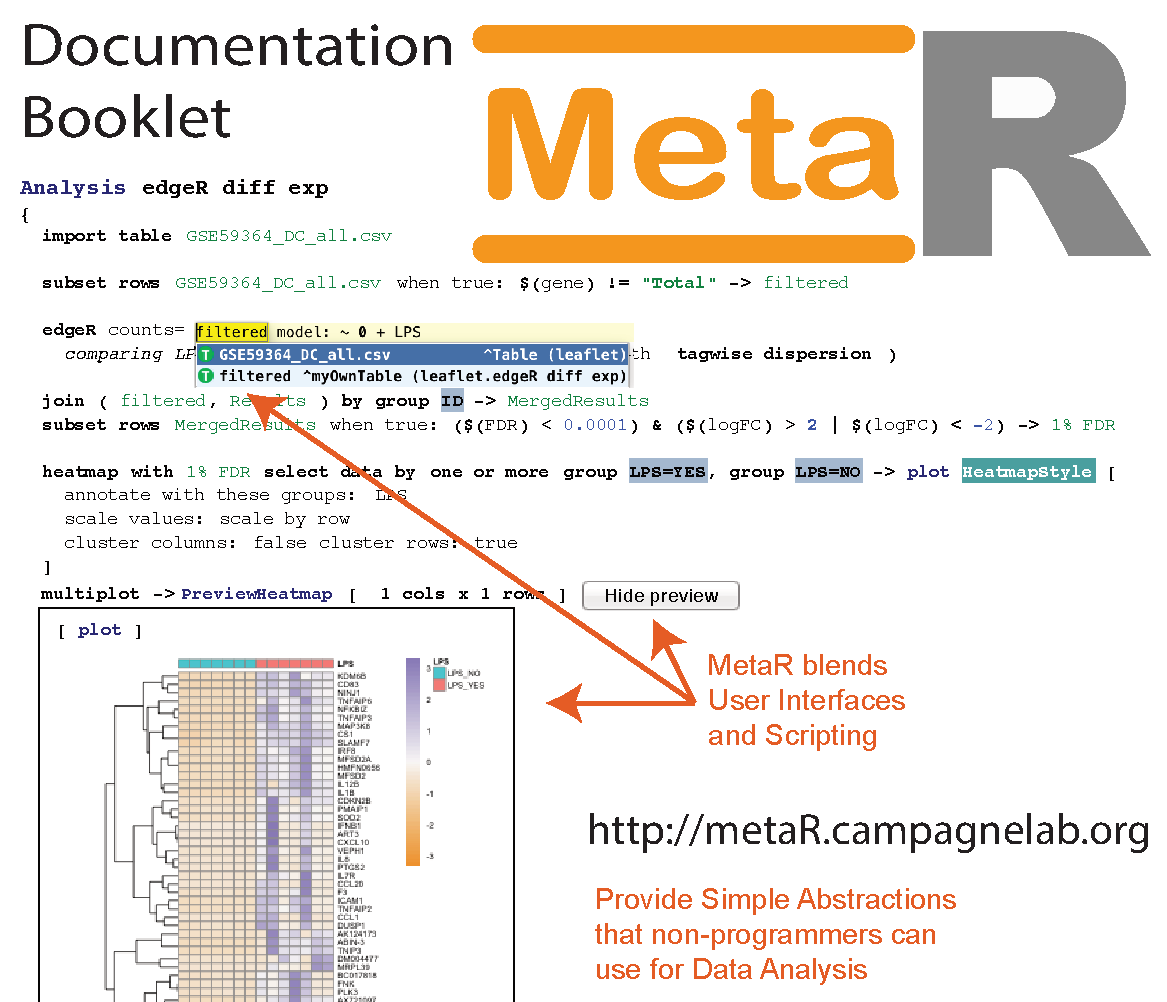
\includegraphics[scale=\coverScalingFactor]{Pictures/MetaRBookCover-v2.pdf}}}} % Image background
\mbox{}
\endgroup
} {
% do not produce a cover/title page
}
%----------------------------------------------------------------------------------------
%	COPYRIGHT PAGE
%----------------------------------------------------------------------------------------

\newpage
~\vfill
\thispagestyle{empty}

\noindent Copyright \copyright\ 2015-2016 Fabien Campagne.\\ % Copyright notice

\noindent \textsc{Published by Fabien Campagne}\\ % Publisher

\noindent \textsc{http://books.campagnelab.org}\\ % URL
\\
\noindent All Rights Reserved. This booklet is licensed under the terms of the Creative Commons 4.0 license (CC BY 4.0, see \url{http://creativecommons.org/licenses/by/4.0}).\\
\noindent Unless required by applicable law or agreed to in writing, software listings provided in this booklet are distributed on an \textsc{``AS IS'' BASIS, WITHOUT WARRANTIES OR CONDITIONS OF ANY KIND}, either express or implied. \\
Reproductions of program fragments from the JetBrains MPS platform are provided in accordance with terms of the Apache 2.0 license. \\
See \url{http://www.jetbrains.com/mps/download/license.html} and\\
\url{http://www.apache.org/licenses/LICENSE-2.0.html}.
\vspace*{0.5cm}


\noindent \textit{Version 1.8.0 April 2016}

% Add an empty page in print edition to put credit on a new leaf
\ifthenelse {\boolean{tablet}}{} 
{\newpage\thispagestyle{empty}\hbox{}}

%----------------------------------------------------------------------------------------
%	CREDITS
%----------------------------------------------------------------------------------------
\newpage\thispagestyle{empty}
\begin{empty}
 \ifthenelse {\boolean{tablet}}{}{
\vspace*{0.15\textheight}
}
\begin{center}\Large{Credits}\end{center}
\normalsize 


The following authors have contributed to this booklet: Manuele Simi, William ER Digan, and Fabien Campagne.


The authors thank the developers of the Meta Programming System, who have developed MPS since the early 2000. MetaR would not have been possible without them. \\
\noindent\textbf{MPS Project leaders, in chronological order:}  Sergey Dmitriev,  Igor Alshannikov, Konstantin Solomatov and Alexander Shatalin. \textbf{Current team members:} Alexander Shatalin, Fedor Isakov, Mihail Muhin, Michael Vlassiev, Václav Pech, Simon Alperovich, Daniil Elovkov, Victor Matchenko, Artem Tikhomirov, Mihail Buryakov and Alexey Pyshkin. \textbf{Earlier members of the MPS team:} Evgeny Gryaznov, Timur Abishev, Julia Beliaeva, Cyril Konopko, Ilya Lintsbah, Gleb Leonov, Evgeny Kurbatsky, Sergey Sinchuk, Timur Zambalayev, Maxim Mazin, Vadim Gurov, Evgeny Geraschenko, Darja Chembrovskaya, Vyacheslav Lukianov and Alexander Anisimov. \textbf{And these external contributors:}  Sascha Lisson, Thiago Tonelli Bartolomei and Alexander Eliseyev.\\

We also thank the many people who have taken the MetaR training sessions at the Clinical Translational Science Center (Weill Cornell Medical College, Memorial Sloan Kettering, and Hospital for Special Surgery and Hunter College). Their feedback we received during these sessions have been instrumental in rapidly making MetaR user-friendly.\\

%\vspace*{\fill}
\end{empty}

\ifthenelse {\boolean{tablet}}{} 
{\newpage\thispagestyle{empty}\hbox{}}

%----------------------------------------------------------------------------------------
%	TABLE OF CONTENTS
%----------------------------------------------------------------------------------------
%latexml \providecommand\chapterimage[1]{#1}
\chapterimage{blue-chapter-head_4-reduced.pdf} % Table of contents heading image

\pagestyle{empty} % No headers

\tableofcontents % Print the table of contents itself

\cleardoublepage % Forces the first chapter to start on an odd page so it's on the right

\pagestyle{fancy} % Print headers again

\newcommand{\MPS}[0]{MPS\index{MPS} }
\newcommand{\AST}[0]{AST\index{AST} }



%\newcommand{\figWidthWide}[0]{16.5cm}
\newcommand{\figWidthWide}[0]{1\textwidth}


%\newcommand{\figWidthNarrow}[0]{10cm}
\newcommand{\figWidthNarrow}[0]{0.66\textwidth}
\newcommand{\figWidthSmall}[0]{0.5\textwidth}
\newcommand{\figWidthTiny}[0]{0.33\textwidth}


\newcommand{\mpsplaceholder}[0]{<<~...~>>}

\newcommand{\mpsImprovementNeeded}[0]{}

\newcommand{\navigateToKeys}[0]{[\keys{\ctrl+N} or \keys{\cmd+N}]}

\newcommand{\mpsDocNotClear}[0]{\index{MPS documentation is not clear}}
%trim option's parameter order: left bottom right top

\newcommand{\intentionLightBulb}[0]{
\includegraphics[trim=0mm 0mm 0mm 0mm, clip,scale=0.5]{Pictures/intentionLightBulb2.png}}

\newcommand{\inspectorTabIcon}[0]{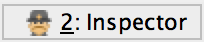
\includegraphics[trim=0mm 0mm 0mm 0mm, clip,scale=0.4]{Pictures/InspectorTabIcon-3.png}}

\newcommand{\tabControlIcon}[0]{
\includegraphics[trim=0mm 0mm 0mm 0mm, clip,scale=0.4]{Pictures/TabControlMPS3_1.png}}


% The following commands do not work.
%\newcommand{\exclamationToDot}[1]{\convertchar{#1}{!}{.}}
%\newcommand{\qualifiedLanguageName}[1]{\convertchar[v]{#1}{.}{\allowbreak{}!}}
%----------------------------------------------------------------------------------------
%	CHAPTERS
%----------------------------------------------------------------------------------------
\ifthenelse {\boolean{fullBook}}{

%----------------------------------------------------------------------------------------
%	CHAP introduction
%----------------------------------------------------------------------------------------

\chapterimage{blue-chapter-head_4-reduced.pdf} % Chapter heading image

\chapter{Introduction}\label{chap:Introduction}
\section{Background}
The MetaR software \url{http://MetaR.campagnelab.org} is an example of a new kind of interactive tool for data analysis. It was developed by my laboratory using the Meta Programming System (MPS) (see \url{http://www.jetbrains.com/mps}~\cite{Dmitriev:2004}. MPS is a mature Language Workbench that makes it relatively easy to create new languages and tools to help users of these languages~\cite{campagne2014mps}. 

\section{Intended audience}
This booklet is designed to teach how to use MetaR for data analysis. In the first chapters, we will assume that you have no prior scripting or programming experience, but will expect you to know how to use a computer.

%TODO re-enable the next sentence when the chapters have been written:
%Chapters~\ref{chap:Intentions}and~\ref{chap:ExtendingMetaR} will be useful for users who also have programming experience. These chapters explain how such users can extend MetaR with intentions or new language constructs.

\section{Key Concepts}
MetaR is designed to make it easier to conduct data analysis. To achieve this goal, and in contrast to programming languages such as the R language, Julia or Python, that are often low-level and require good programming skills, MetaR offers high-level data abstractions and provides assistance in manipulating data. High-level abstractions used in MetaR analyses include the following concepts:

\begin{enumerate}
	\item Tables, Columns, Column Groups and Group usages,
	\item Plot
	\item Model
\end{enumerate}

\noindent{}These high-level abstractions will be explained in the following chapters.

\section{Solutions and Models}
Developing an analysis with MetaR is done by creating nodes of the MetaR concepts in MPS models. Models exist in MPS solutions. To learn how to create an MPS solution, read the preview of the MPS language workbench available at \url{http://campagnelab.org/publications/our-books/}\cite{campagne2014mps}, or watch the beginning of the MetaR training video at \url{http://campagnelab.org/software/metar/video-tutorials/}. Figures~\ref{fig:QuickStartMenu}-\ref{fig:NewProjectDialog} provide a brief walk-through of the steps you should follow to create a project and solution. After the project open, open the project tab(see ~\cite{campagne2014mps}) and right-click on the solution name. Import the metaR devkit and create a model. 

You can create as many models as you need to store your analyses. In the following chapter, we assume that you have created a solution and at least one model in this solution. 


\begin{SCfigure}
  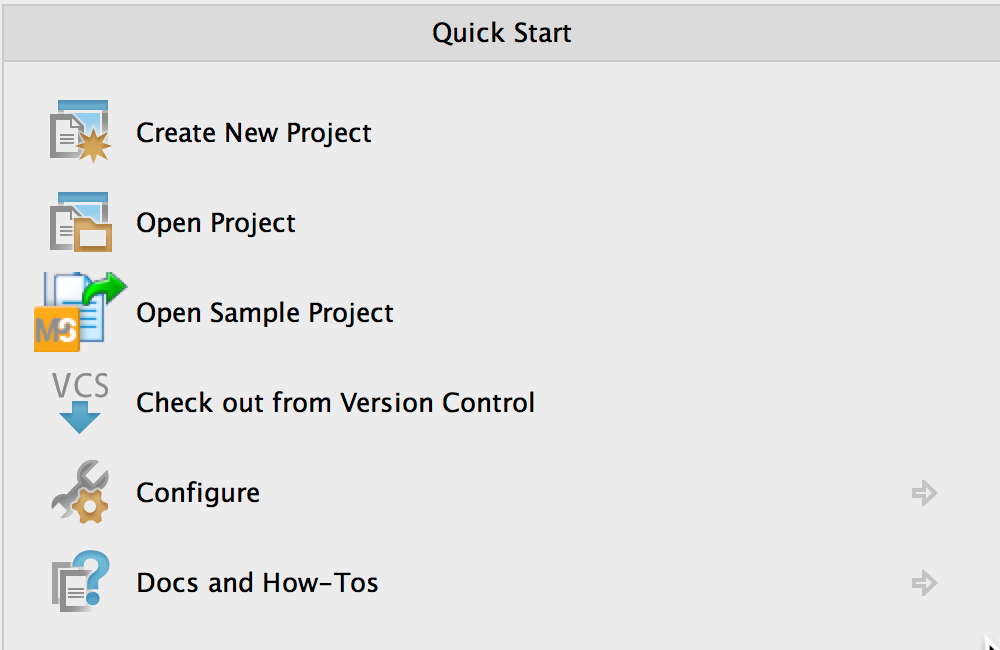
\includegraphics[width=\figWidthNarrow]{figures/QuickStart.png}
  \caption[The Quick Start menu.]{\textbf{The Quick Start menu.} This menu is displayed when you first open MPS, or when you have no project currently open in MPS. The first item in the menu is used to create a new project. 
}\label{fig:QuickStartMenu}
\end{SCfigure}

\begin{SCfigure}
  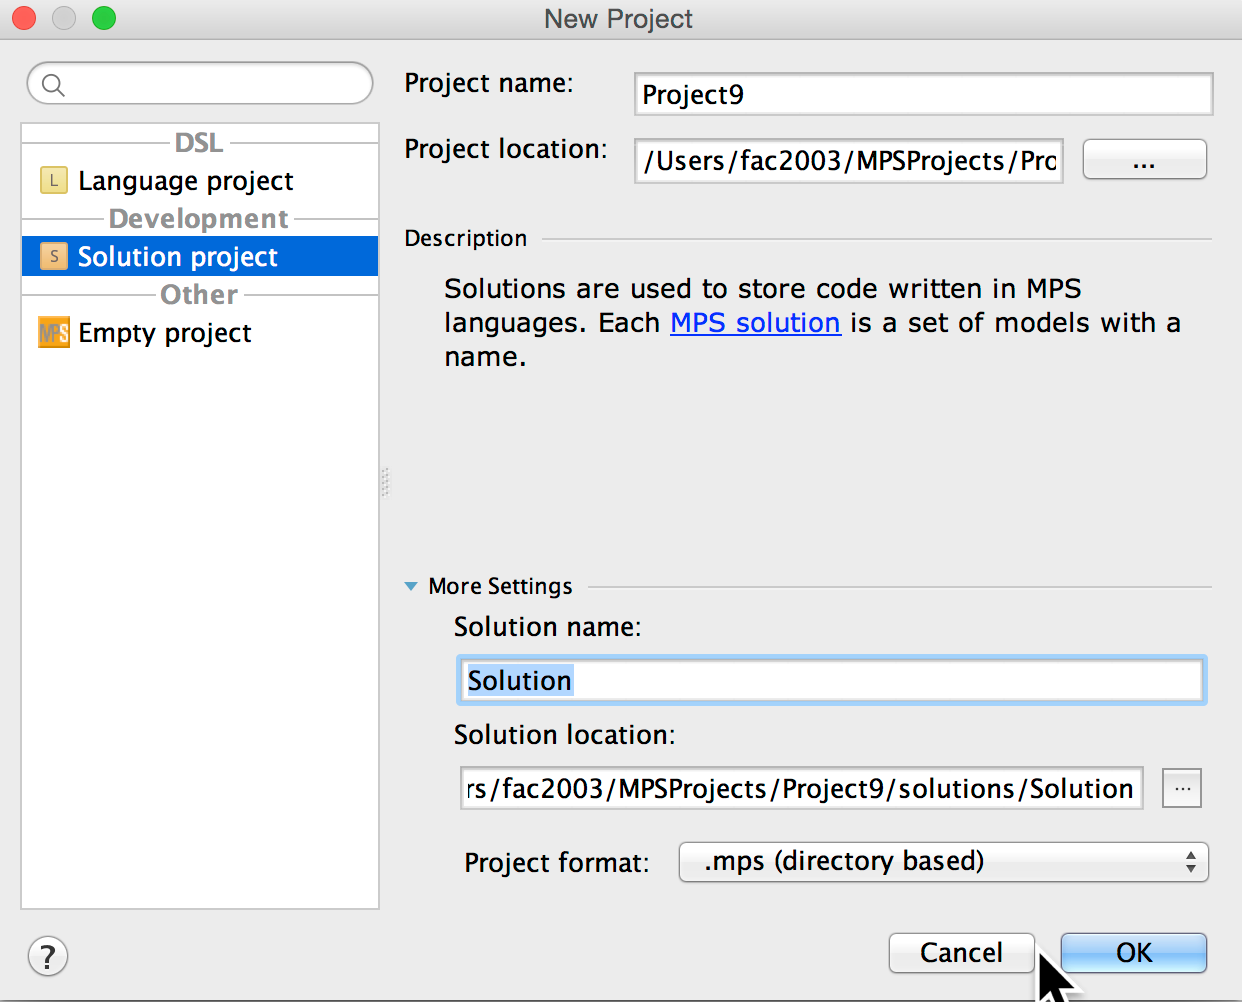
\includegraphics[width=\figWidthNarrow]{figures/NewSolutionWizard.png}
  \caption[The New Project Dialog.]{\textbf{The New Project Dialog.} Use this dialog to create a new Solution. Solutions are used to store models and express your solutions to specific analysis problems. Select the ``Solution Project'' project type on the left panel, name the project, and name the solution you wish to create.
}\label{fig:NewProjectDialog}
\end{SCfigure}


%----------------------------------------------------------------------------------------
%	CHAP introduction
%----------------------------------------------------------------------------------------

\chapterimage{blue-chapter-head_4-reduced.pdf} % Chapter heading image

\chapter{Tables}\label{chap:Tables}
\section{Overview}
Before you start an analysis, you will need to define Table nodes that represent the data files needed in the analysis. MetaR explicitly models files that contain tables of data. This is done so that you can easily refer to these tables, without having to remember where the original file is located on your computer. 

\noindent In this Chapter, you will learn how to 
\begin{enumerate}
	\item define a MetaR table,
	\item  adjust the types of the columns of the data described in the file,
	\item annotate a table with groups,
	\item link groups in column group usage.
\end{enumerate}

\section{Create a Table}\label{sec:CreateATable}\index{Create a Table}
To create a Table, right-click on a model in the project tab and select \menu{right-click > New > o.c.metar.tables > Table}. This will create an empty table, as shown in Figure~\ref{fig:NewTable}. Tables have a \texttt{name}, a \texttt{pathToResolve} attribute and a list of columns. The following paragraphs describe these attributes.
\paragraph{name}
The table name is set automatically from the path when you use the file selection button. You can change the name to match your analysis needs and make it easier to remember what is in the table.
\paragraph{File Path (pathToResolve)}
This attribute contains a path to the TSV file that you wish to analyze. The path may contain references to path variables that will be automatically resolved before MetaR attempts to load table information from the path. Path variable references can be written as \texttt{\${a.b.c}/data/file.tsv}. Such a reference will require you to define the a.b.c path variable name and associate it with a value on each machine where the table will be used. You can define path variables with the Preferences/Settings MPS menu (\menu{MPS > Preferences> PathVariables} on Mac, \menu{MPS > Settings > PathVariables} on PC).

\paragraph{Columns}
Columns is an attribute that presents the list of columns identified in the TSV file. Each column has a name, a type, and may be annotated with a set of column groups (see Section~\ref{sec:ColumnGroups} for details about column groups).
MetaR supports the following column types, which map to the R data types:
\begin{enumerate}
	\item \textbf{Numeric}. Any number. Technically, can be a floating number or an integer.
	\item \textbf{String}. A string of characters.
	\item \textbf{Boolean}. A type that can only have two values: \texttt{true} or \texttt{false}.
	\item \textbf{Category}. A type that can take only a limited number of values (e.g., \{\texttt{RED}, \texttt{GREEN}, \texttt{BLUE}\} would be a category with these values, (\texttt{RED}, \texttt{GREEN} and \texttt{BLUE} in our example).
\end{enumerate}
These types are automatically determined from the data in the table file. However, in case the automatic algorithm failed for a table, you can change the types manually. To do this, put the cursor over the name of the type in the column section, and use auto-completion in the inspector to change to the desired type.
 
\begin{SCfigure}
  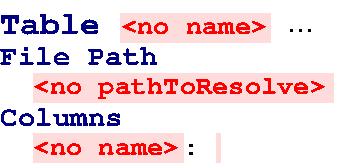
\includegraphics[width=\figWidthTiny]{figures/NewTable.pdf}
  \caption[New Table.]{\textbf{New Table.} This figure presents a freshly created Table AST Root node. You can use the button located to the right, after the <no name> red label (\keys{...}), to open a file selection dialog. Use this dialog to locate a TSV file to configure this table.}\label{fig:NewTable}
\end{SCfigure}

Figure~\ref{fig:ExampleTable} presents a MetaR table annotated with groups. \index{Example}

\begin{figure}[h!tbp]
  \centering
  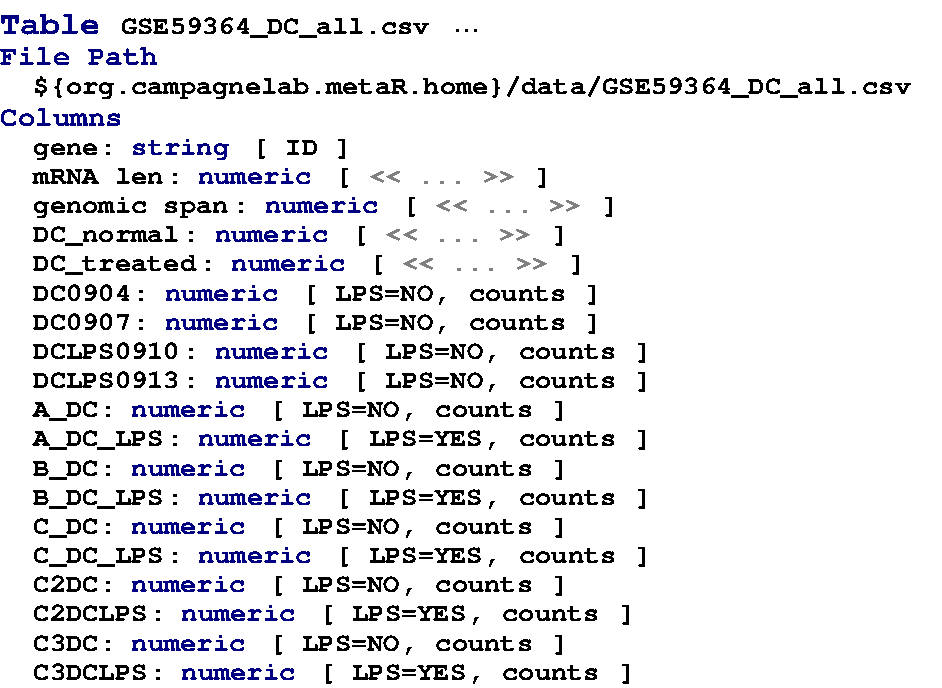
\includegraphics[width=\figWidthWide]{figures/ExampleTable.pdf}
\caption[Example Table.]{\textbf{Example Table.} The figure presents an example table annotated with groups.}
\label{fig:ExampleTable}
\end{figure}


\section{Column Groups Container}\label{sec:ColumnGroupContainer}\index{Column Groups Container}
Column Groups Containers are used to define column groups and annotate these groups with group usages.
To create a new Column Group Container, right-click on a model and select \menu{New > o.c.tables.ColumnGroupContainer}. This will create the empty container shown in Figure~\ref{fig:NewColumnGroupContainer}. You need and should have only one container per model. The container will hold the groups and group usages that you need across the MetaR Tables defined in the model.
\begin{SCfigure}
  \centering
  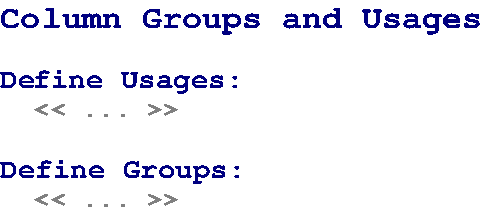
\includegraphics[width=\figWidthNarrow]{figures/NewColumnGroupContainer.pdf}
\caption[Empty Column Group Container.]{\textbf{Empty Column Group Container.} Use a column group container to define column groups and associated group usages. Place the cursor over the \mpsplaceholder{} symbol and press \keys{\return} to add a new group or group usage. Name the group or usage immediately after creating it.}
\label{fig:NewColumnGroupContainer}
\end{SCfigure}

\section{Column Groups}\index{Column Groups}\label{sec:ColumnGroups}
Column Groups can be defined by pressing \keys{\return} either on top of the \mpsplaceholder{} (immediately below \texttt{Define Groups:}), when the list of groups is empty, or with the cursor immediately before the name of an existing group. Each group has a name and an optional set of group usages. Figure~\ref{fig:NewGroup} presents a new column group (group for short).

\begin{SCfigure}
  \centering
  
\includegraphics[width=\figWidthNarrow]{figures/NewGroup.pdf}
\caption[New Group.]{\textbf{New Group.} You should name a new group immediately after creating it.}
\label{fig:NewGroup}
\end{SCfigure}

\paragraph{name} The name of the group is a string that should mean something in the context of your analysis. Some MetaR analysis statements require specific group names to be defined in a model container and referenced in an input table. Other groups will be created by you with meaningful names to help identify columns that have certain properties, so that you can refer to them collectively by the group name. 

\paragraph{used for}
Column groups can be annotated with a set of group usages. You can enter references to usages already defined in the column group container following the \texttt{used for} keyword shown in Figure~\ref{fig:NewGroup}. Press \keys{\enter} on the \mpsplaceholder{} to insert the first group usage. Make sure the usage is defined (its name should be visible in the \texttt{Define Usages:} section of the container (see Section~\ref{sec:ColumnGroupUsage} to lean how to create a new Group Usage). You can bind a group usage reference to a Group usage by using auto-completion (\keys{\ctrl+\space} to locate the name, then pressing \keys{\enter} to accept one completion choice), or by typing the name of the group usage directly (note that group usage names are case sensitive).

\begin{remark}
	Pressing \keys{\return} before \texttt{<no name>} will not have the desired effect if you have not yet named a group. Make sure you name groups immediately after you create them. 
\end{remark}

 
\section{Column Group Usage}\label{sec:ColumnGroupUsage}
A Column Group Usage can be defined by pressing \keys{\return} either on top of the \mpsplaceholder{} (immediately below \texttt{Define Usages:}), when the list of group usages is empty, or with the cursor immediately before the name of an existing group usage. When the list already contains one or more group usages, you can add more by placing the cursor over a group usage name and pressing \keys{\enter}. Keep pressing \keys{\enter} to add more empty group usages.

\section{Example Column Group Container}\index{Example}
Figure~\ref{fig:ExampleGroupContainer} presents an example of a configured Column Group Container. This container defines two groups \texttt{LPS=yes} and \texttt{LPS=no}, which can be used to annotate Table columns that contain data about gene expression of samples treated with LPS or not.  The group usage \texttt{LPS\_Treatment} is associated to both groups to indicate that they belong together and are two kinds of treatment.

\begin{SCfigure}
  \centering
  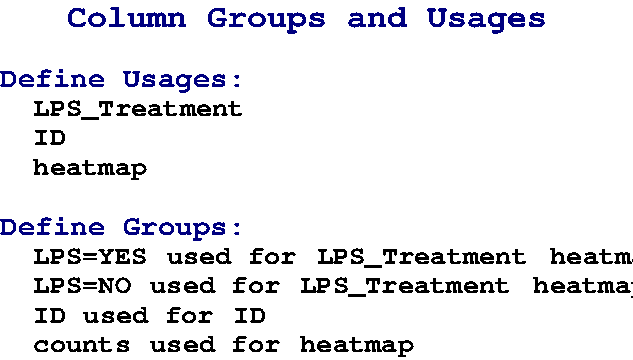
\includegraphics[width=\figWidthNarrow]{figures/ExampleGroupContainer.pdf}
\caption[Example Group Container.]{\textbf{Example Group Container.} This example presents a container with several groups and group usages.}
\label{fig:ExampleGroupContainer}
\end{SCfigure}


%----------------------------------------------------------------------------------------
%	CHAP Analysis
%----------------------------------------------------------------------------------------

\chapterimage{blue-chapter-head_4-reduced.pdf} % Chapter heading image

\chapter{Analyses}\label{chap:Analyses}


\section{The MetaR Analysis Root Node}
MetaR analyses are represented with an Analysis AST Root node. An analysis often imports one or more tables, performs data transformations and writes a table or generates some plots. 
You can create as many Analysis root nodes as needed in a model. You create an analysis by right-clicking on a model and selecting \menu{New > o.c.metar.tables > Analysis}. Analysis can exist as direct child of a model, and for this reason is called a root node. Figure~\ref{fig:NewAnalysis} presents a new Analysis root node. 

\begin{SCfigure}
  \centering
  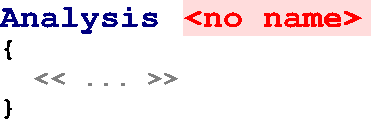
\includegraphics[width=\figWidthTiny]{figures/NewAnalysis.pdf}
\caption[New MetaR Analysis Root Node.]{\textbf{New MetaR Analysis Root Node.} This figure presents a freshly created MetaR analysis root node. You can press \keys{\return} over the \mpsplaceholder{} to add Statement nodes to the analysis. Use auto-completion to discover which types of statements are available. }
\label{fig:NewAnalysis}
\end{SCfigure}

\paragraph{name}
Each analysis has a name. You should name the analysis after creating it. The name you enter will be shown in the Project Tab after the 
\includegraphics[height={2ex}]{figures/analysis.png} icon.

\paragraph{statements}
An analysis contains a list of statements. You can enter new statements by typing between the curly brackets \texttt{\{} \texttt{\}}. 

To enter a specific statement, you can type the \texttt{alias} of the statement (for instance \texttt{import table}). When you have typed a complete alias, the node will be inserted in place of the alias. Note that there is no actual indication that the text you are typing matches a valid alias. You need to finish typing the full alias before the node is substituted for the alias. The text you type will remain red until the substitution occurs even if the text is matching a valid alias. See Figure~\ref{fig:TypingStatementAliases}.

\noindent The following sections describe the kinds of statements offered by the MetaR \texttt{org\allowbreak.campagnelab\allowbreak.MetaR\allowbreak.tables} language. The simplest way to learn which statements are supported by the release of MetaR that you are using is to use auto-completion. Figure~\ref{fig:AutoCompletionForStatements} provides a snapshot of the auto-completion menu when looking for statements to insert in the Analysis statement list. 
\begin{figure}[h!tbp]
  \centering
  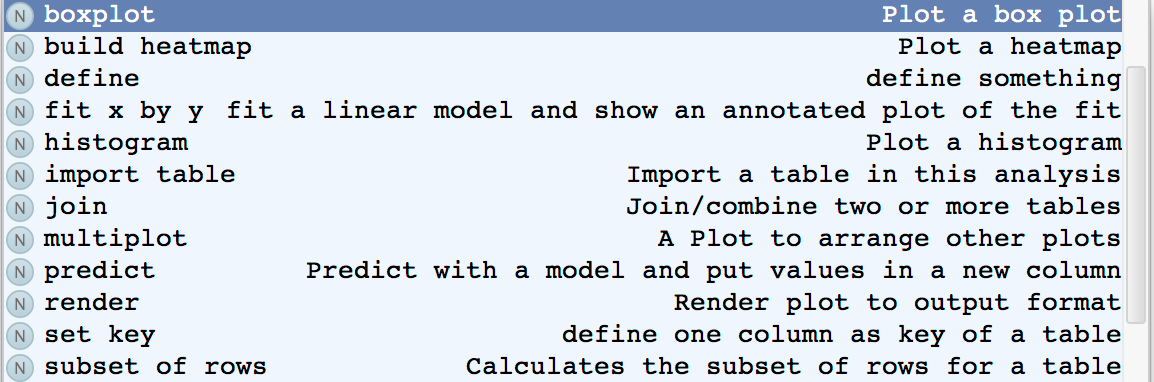
\includegraphics[width=\figWidthWide]{figures/StatementAuto-completion.png}
\caption[Auto-completion Dialog for Statements.]{\textbf{Auto-completion Dialog for Statements.} This dialog is obtained by placing the cursor where a Statement is valid, and pressing \keys{\ctrl+\space}.}
\label{fig:AutoCompletionForStatements}
\end{figure}



\begin{figure}[h!tbp]
  \centering
  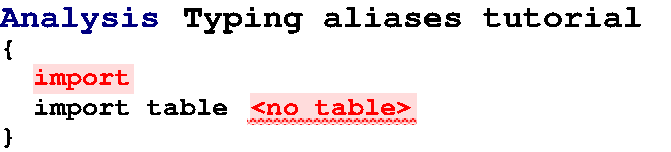
\includegraphics[width=\figWidthNarrow]{figures/AnalysisTypingAliases.pdf}
\caption[Typing Statement Aliases.]{\textbf{Typing Statement Aliases.} The user has typed ``import'' on the third line. This text is a prefix of the import table statement, but is shown in red because the alias is not yet complete. The fourth line shows the import statement which is substituted to the text when the user has just finished typing ``import table'', the complete alias of the statement. Note that pressing \keys{\return} immediately after import will create the node if the prefix ``import'' matches a single type of node in the languages imported in this model.}
\label{fig:TypingStatementAliases}
\end{figure}

\section{Working with Tables}

\subsection{Import Table}
The \texttt{import table} statement makes it possible to import a table, defined in the model, into the analysis. The columns of the imported table will become visible to the statements that follow the import. You can create an import table statement by typing the alias \texttt{import table} on an empty line of Analysis. Once you have bound the reference to a table, the import statement will look like this: 
\includegraphics[height=2ex]{figures/SomeDataImportTable.pdf}. The name in green is the name of the table the statement imports. See Section\ref{sec:CreateATable} to learn how to create a Table Root node.
\paragraph{table}

The table attribute is a reference to an AST root node. You can set this reference by typing the name of the table you wish to import, or by using auto-completion \keys{\ctrl+\space} to locate the table AST root node.

\subsection{Write Table}
MetaR analyses can create new tables. You can write the data in these tables to a file using the \texttt{write} statement (see Figure~\ref{fig:NewWriteTableStatement} for a new write statement). The write statement has two attributes: table and filename.
\begin{SCfigure}
  \centering
  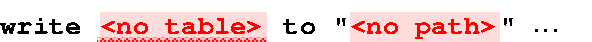
\includegraphics[width=\figWidthNarrow]{figures/NewWriteStatement.pdf}
\caption[New Write Statement	.]{\textbf{New Write Statement.} Use this statement to write the content of a table to a file.}
\label{fig:NewWriteTableStatement}
\end{SCfigure}


\paragraph{table}
This reference should be set to the table that you want to write to a file.
\paragraph{output}
The output should be set to a filename where you want the data contained in the table to be written. Notice that output has a button to let you select the output filename.

\section{Subset Rows}
You can use this statement (alias \texttt{subset rows}) to filter a table and produce a new table with a subset of the rows of the input table. Figure~\ref{fig:NewSubsetRows} shows a new \texttt{subset rows} statement.

\begin{SCfigure}
  \centering
  
\includegraphics[width=\figWidthNarrow]{figures/NewSubsetRowsStatement.pdf}
\caption[New Subset Rows Statement.]{\textbf{New Subset Rows Statement.} Use this statement to filter the rows of a table.}
\label{fig:NewSubsetRows}
\end{SCfigure}

\paragraph{table}
The input table reference must be set to a table. The table must be either imported or produced by another statement.
\paragraph{filter}
The filter determines which rows are kept. Use auto-completion to select one of the alternatives:
\begin{enumerate}
	\item \texttt{when true:} will keep a row when the boolean expression following when \texttt{true:} evaluates to  \texttt{true}.
	\item \texttt{with IDS} will keep a row when the value of the column marked with group \texttt{ID} exists in the list provided as an argument. See the \texttt{define} statement to create a list of IDs. 
\end{enumerate}

\paragraph{subset}
The output table is called subset by default. Feel free to rename this table to better match the data in it.

\subsection{Example}
Figure~\ref{fig:ExampleSubsetRows} presents examples of subset row statements. 

\begin{figure}[h!tbp]
  \centering
  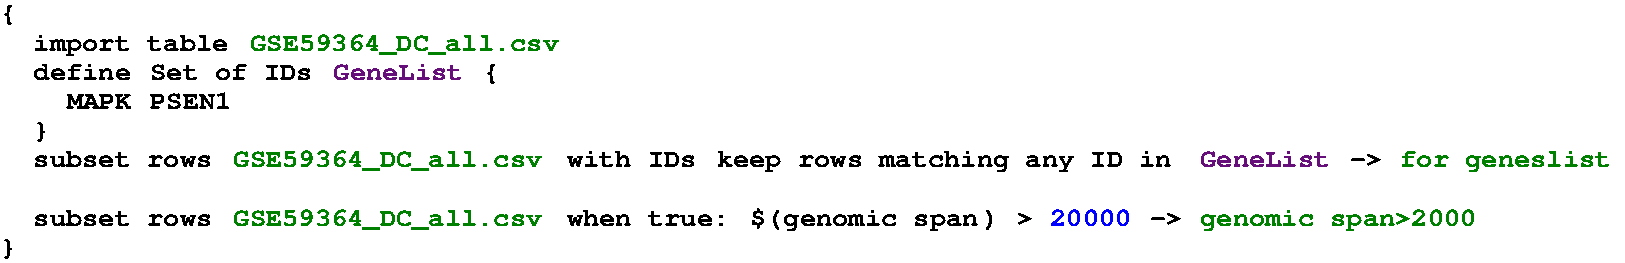
\includegraphics[width=\figWidthWide]{figures/ExampleSubsetRows.pdf}
\caption[Subset Rows Examples.]{\textbf{Subset Rows Examples.} This figure illustrates the two alternatives available for filtering rows: by expression (with \texttt{when true:}, or with a set of ID values).}
\label{fig:ExampleSubsetRows}
\end{figure}

\subsection{Boolean Expressions}
One form of the subset rows statement accepts a boolean expression to determine which rows to keep. Boolean expression have one of two values: true or false, and can be constructed by comparing values with an operator. The following operators are supported by MetaR:
\begin{itemize}
 \item \textbf{\$(} column \textbf{)} The value operator evaluates to the value of the column in the row currently considered.
	\item expr1 \textbf{==} expr2 true when expr1 evaluates to the same value as expr2.
	\item expr1 \textbf{!=} expr2 true when expr1 does not evaluate to the same value as expr2.
	\item expr1 \textbf{|} expr2 true when expr1 is true or expr2 is true (boolean or. either one of expr1 or expr2 needs to be true for the result to be true).
    \item expr1 \textbf{\&} expr2 true when expr1 is true and expr2 is true (boolean and, both expre1 and epr2 must be true for the result to be true).
    \item expr1 \textbf{<} expr2 true when expr1 evaluates to a value less than expr2.  
    \item expr1 \textbf{>} expr2 true when expr1 evaluates to a value greater than expr2.  
   \item expr1 \textbf{<=} expr2 true when expr1 evaluates to a value less or equal than expr2.  
    \item expr1 \textbf{>=} expr2 true when expr1 evaluates to a value greater or equal than expr2.  
\end{itemize}

\begin{remark}
MetaR infers the type of the expressions that you enter and will report type errors if the value of some values are not compatible with the test that your perform.
\end{remark}

\section{Join Tables}
When you perform data analysis, you often need to combine data from different tables into one. This operation is called table joining. MetaR provides a powerful \texttt{join} statement that helps join an arbitrary number of tables. The alias of the statement is \texttt{join}. Figure~\ref{fig:NewJoinStatement} presents a newly created \texttt{join} statement. Join has three attributes: input tables, by and output table.

\begin{SCfigure}
  \centering
  
\includegraphics[width=\figWidthNarrow]{figures/NewJoinStatement.pdf}
\caption[New Join Statement.]{\textbf{New Join Statement.} Use this statement to join two or more tables into one.}
\label{fig:NewJoinStatement}
\end{SCfigure}

\paragraph{input tables}
Use this attribute to enter references to tables you need to join. You can press \keys{\return} with the cursor inside the parentheses to create references to additional input tables.
\paragraph{by}
Use the by attribute to specify how to join the input tables. Joining tables require knowing which rows of the input tables go together. MetaR supports three strategies:
\begin{itemize}
	\item \textbf{by columns:} Use the set of columns provided here. The same column name must be defined in all the input tables.
	\item \textbf{by group:} Use the set of columns annotated with this group. As long as each table has one or more columns annotated with this group, the name of the columns do not need to be the same. 
	\item \textbf{by groups:} Use the set of columns annotated with any of these groups. Similar to group, but with any (>=1) number of groups. Press \keys{\return} to insert new group references.
\end{itemize}

Each strategy identifies a set of columns. The group by columns are used to calculate a list of values. When rows of the input tables have the same group by values, they are joined in a single row, and the result put in the destination table. 

\begin{remark}
The join statement will create new columns if the input tables have column with the same name. In this case the shared columns are renamed ``colanme.TableName''. Place the cursor of result and look at the column preview in the inspector to see which column names are generated by a given join.
\end{remark}

\paragraph{result}
The output table is called Results by default. Feel free to rename this table to match the content of the destination table. Open the \inspectorTabIcon{} to see which columns will result from the join. Notice that the column groups are transfered to the columns of the output table.


\subsection{Example Join}
Figure~\ref{fig:ExampleJoinStatement} presents an example of join statement. The statement joins two tables and creates the Result table. If you open the \inspectorTabIcon{}, you will see a preview of the columns for the result table (shown in Figure~\ref{fig:ColumnPreviewExample}). 
\begin{SCfigure}
  \centering
  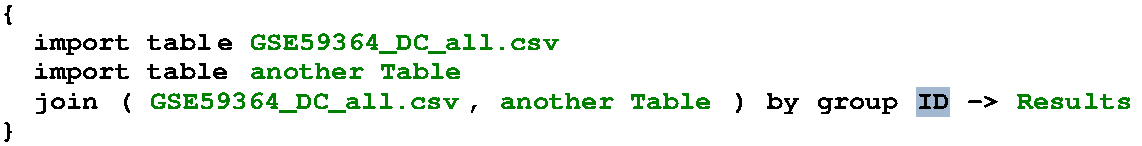
\includegraphics[width=\figWidthNarrow]{figures/ExampleJoin.pdf}
\caption[Example of Join Statement.]{\textbf{Example of Join Statement.}}
\label{fig:ExampleJoinStatement}
\end{SCfigure}


\begin{figure}[h!tbp]
  \centering
  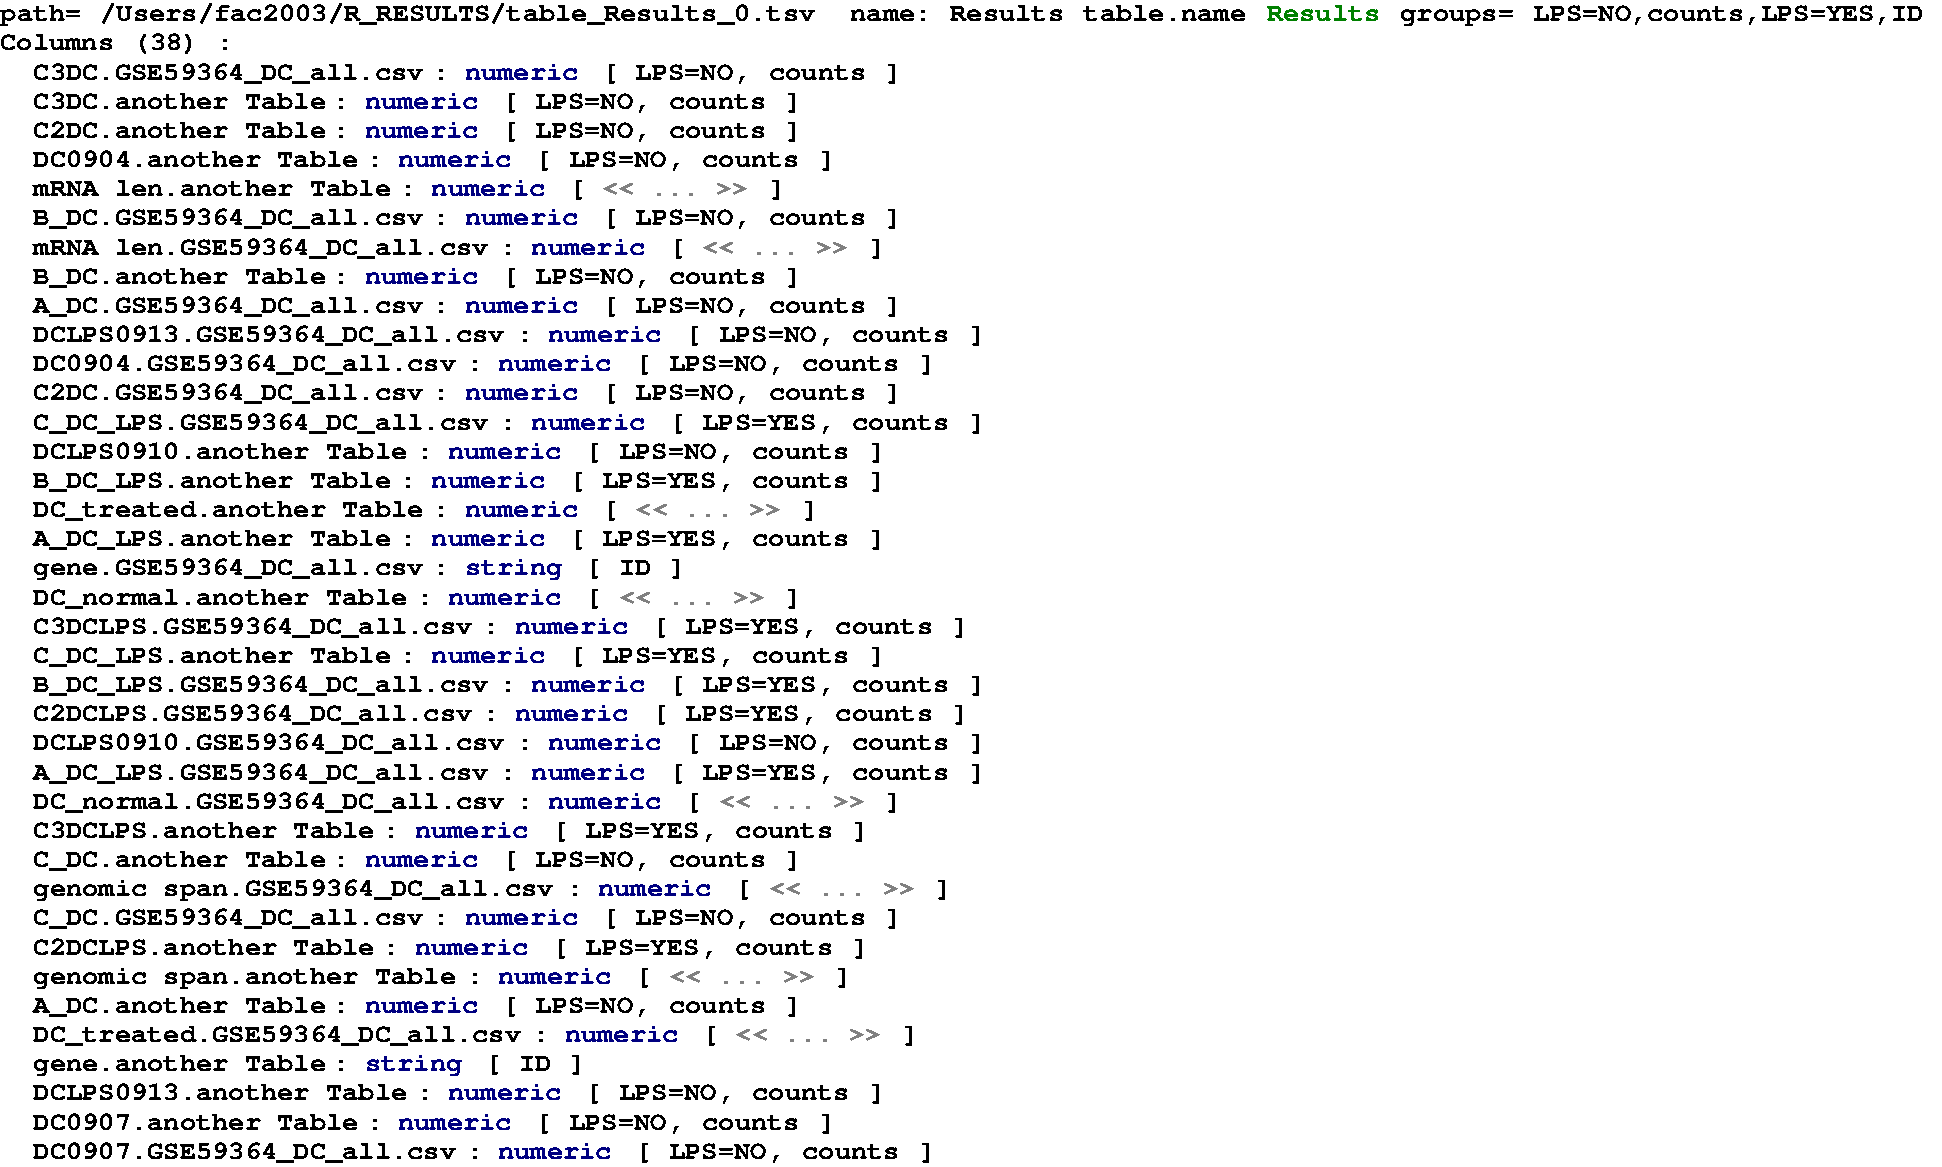
\includegraphics[width=\figWidthWide]{figures/ExampleJoinColumnPreview.pdf}
\caption[Column Preview for Result Table.]{\textbf{Column Preview for Result Table.} Notice that all these columns were shared across the input tables because their name follows the pattern ``colName.tableName''.}
\label{fig:ColumnPreviewExample}
\end{figure}


\section{Plotting Data}
MetaR provides simple plotting capabilities\footnote{These capabilities are simple, but can be extended very easily by adding new statements to draw other types of visualizaton. This is a key advantage of using Language Workbench technology.}. The following types of plots are currently supported: 
\begin{itemize}
  \item boxplot alias \texttt{boxplot}
  \item histogram alias \texttt{histogram}
  \item scatterplot: alias \texttt{fit}
  \item heatmap, alias \texttt{build heatmap}
  \item multiplot alias \texttt{multiplot}, makes it possible to organize other plots in a matrix of n columns by n rows.
\end{itemize}

\subsection{boxplot}
Figure~\ref{fig:NewBoxPlot} presents a new boxplot statement.

\begin{SCfigure}
  \centering
  
\includegraphics[width=\figWidthNarrow]{figures/NewBoxplot.pdf}
\caption[New Boxplot Statement.]{\textbf{New Boxplot Statement.}}
\label{fig:NewBoxPlot}
\end{SCfigure}

\paragraph{columns}
Indicate one or more columns to plot. The values of the columns will be plotted as individual boxplots in the same graph. Press \keys{\enter} to define more than one column. Use auto-completion to locate individual columns from the imported tables, or the tables created by prior statements. 

\paragraph{plot}
The attribute after \texttt{->} is a plot. Enter a name for the boxplot here. Plot names are colored blue to make them easier to recognize.

\paragraph{style}
Different kind of plots accept different types of styles. The boxplot accepts a \texttt{Color\allowbreak{}Plot\allowbreak{}Style}. You can create this node in the model and bind the boxplot statement to it to customize the colors that will be used to draw this boxplot. 


\subsection{histogram}
Use this statement to plot a histogram of the values of one column.
\paragraph{column}
Indicate one to plot a histogram for.  Use auto-completion to locate the column from the imported tables, or the tables created by prior statements. 

\paragraph{plot}
The attribute after \texttt{->} is a plot. Enter a name for the histogram here. Plot names are colored blue to make them easier to recognize.

\paragraph{style}
Different kind of plots accept different types of styles. The histogram accepts a \texttt{Color\allowbreak{}Plot\allowbreak{}Style}. You can create this node in the model and bind the histogram statement to it to customize the colors that will be used to draw this plot. 



\subsection{fit x by y}
Use this statement (alias \texttt{fit}) to plot a scatter plot of x (one column) vs y (another column). A fit is performed, and the R2 adjusted, and P-value corresponding to the linear regression is shown on the plot. Figure~\ref{fig:NewFitXByY} presents a new \texttt{fit} statement.

\begin{figure}[h!tbp]
  \centering
  
\includegraphics[width=\figWidthWide]{figures/NewFitXByY.pdf}
\caption[New Fit X by Y.]{\textbf{New Fit X by Y.}}
\label{fig:NewFitXByY}
\end{figure}

\paragraph{x, y}
Indicate which columns should be plotted. Use auto-completion to locate the x and y columns from the imported tables, or the tables created by prior statements. 

\paragraph{plot}
The attribute after \texttt{->} is a plot. Enter a name for the scatterplot here. Plot names are colored blue to make them easier to recognize.

\paragraph{style}
Different kind of plots accept different types of styles. The fit statement accepts a \texttt{Scatter\allowbreak{}Plot\allowbreak{}Style}. You can create this node in the model and bind the fit statement to it to customize the title, axes and range of data in the scatterplot. Figure~\ref{fig:NewScatterPlotStyle} shows the attributes of the \texttt{ScatterPlotStyle} node.


\begin{SCfigure}
  \centering
  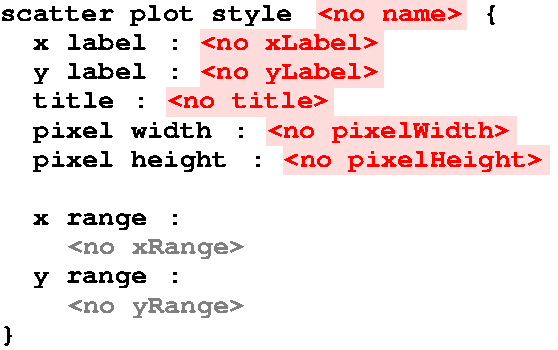
\includegraphics[width=\figWidthNarrow]{figures/NewScatterPlotStyle.pdf}
\caption[New Scatterplot Style.]{\textbf{New Scatterplot Style.}}
\label{fig:NewScatterPlotStyle}
\end{SCfigure}









%	CHAP Docker%----------------------------------------------------------------------------------------

\chapterimage{blue-chapter-head_4-reduced.pdf} % Chapter heading image

\chapter{Docker Integration}\label{chap:DockerIntegration}
The integration with Docker helps with the reprducibility of your analyses. Installing packages with R does not make it possible to specific exactly the version of the package that you need for an analysis. While it is possible to always install the latest version of a package, the behavior of some packages will change over time. For this reason, it is useful to build snapshots of the R packages used during analysis and report the version number of the snapshot. 

\section{Pre-requisites}
You will need a working docker installation on your machine before you can run MetaR analyses with Docker (see \url{http://docs.docker.com/installation/}).

\subsection{Mac OS}
Mac users will find it convenient to download and install the docker native installation. After installation, open a Terminal and type 
\texttt{docker pull fac2003:rocker-metar:latest} 

\subsection{Other Platforms}
Other users should refer to documented installation steps for their platform.

\section{Configuring Docker}\index{Docker}
Docker integration can be configured using the MPS Preferences.  Open Preferences (Setting on Windows) and locate the Docker configuration (use the search box with the docker keyword). You will be presented with the following dialog shown in Figure~\ref{fig:DockerPreferencesDialog}.

\begin{figure}[h!tbp]
  \centering
  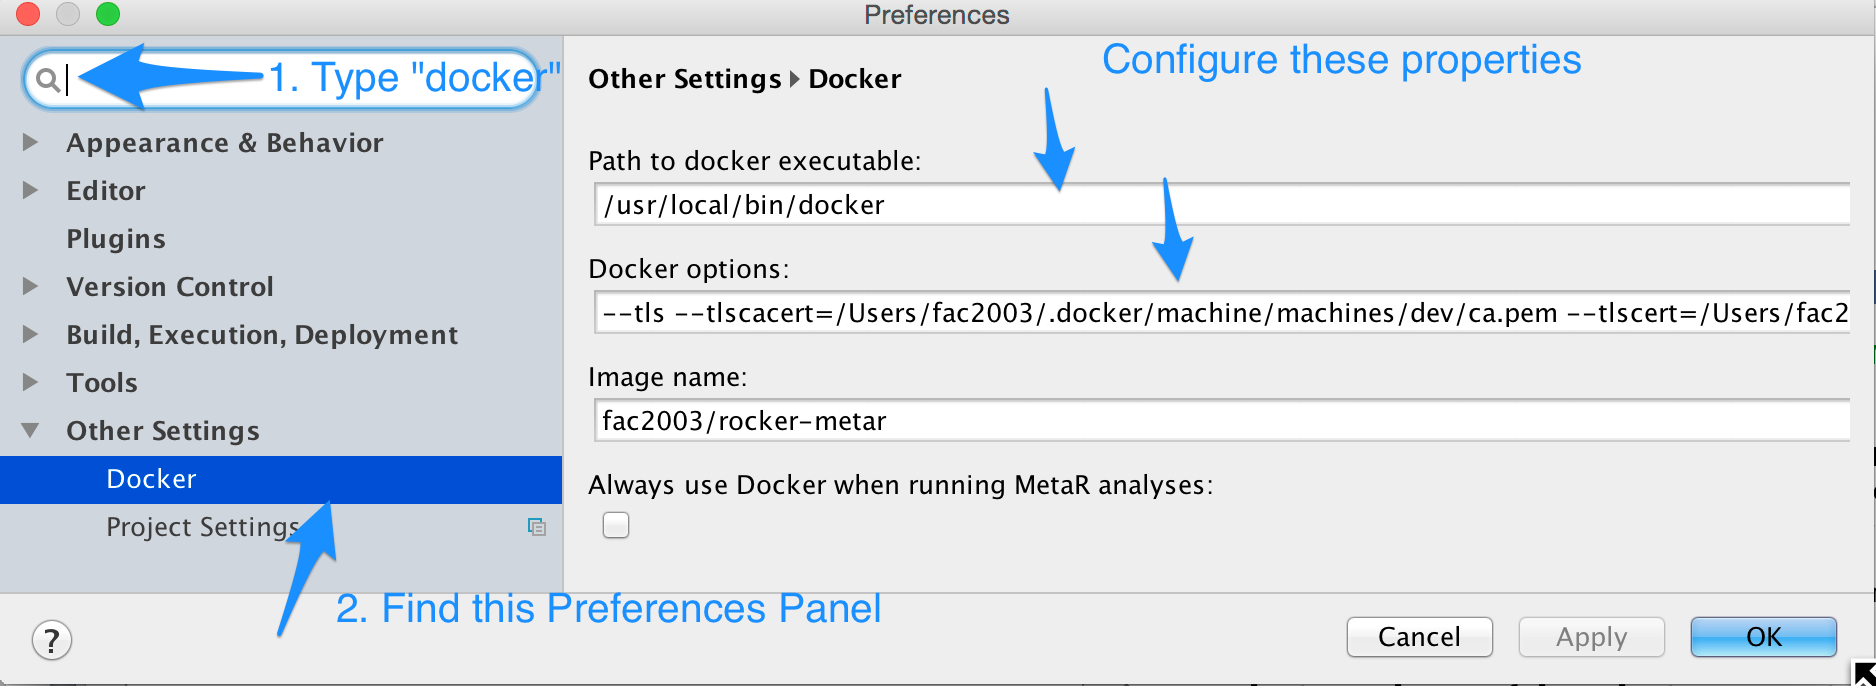
\includegraphics[width=\figWidthWide]{figures/DockerPreferencesDialog.png}
\caption[Docker Configuration Dialog.]{\textbf{Docker Configuration Dialog.} This dialog is available under MPS Preferences/Settings.}
\label{fig:DockerPreferencesDialog}
\end{figure}

\paragraph{path to docker executable}
This field must provide a path to a valid docker executable. On linux, try \texttt{which docker} in the shell. On Mac, start a Terminal and type \texttt{which docker} and copy the location to the field. 

\paragraph{docker options}
These are the options necessary to connect to the docker server. If you installed  docker native, you don't need to enter any options.  On other platforms, open the docker application and start the terminal with the \menu{File>Open Docker Command}\allowbreak\menu{Line Terminal Window}. In the window, type \texttt{echo `docker-machine config`} and copy the line printed to the field. 


\paragraph{image name}
This is the name of the docker image that you wish to use with MetaR. Keep the default, or enter a customized image name here. Customizing the image is useful if you need to install additional packages than the ones we use during our training sessions. If you create a new image, make sure you use \texttt{fac2003/rocker-metar} in the FROM field. Images that do not build on \texttt{fac2003/rocker-metar} are not supported at this time. 

\begin{remark}
Note that you can specify an image tag/version number. Append a colon (:) and the tag after the image name. For instance, use \texttt{fac2003/rocker-metar:2.1.0} to run the \texttt{rocker-metar} image packaged with MetaR 2.1.0.  
\end{remark}

\begin{remark}
Note that specifying a tag is a good idea if you need to reproduce exactly an analysis in the future. Omitting the tag will always get the latest version of the image, which may change over time.  
\end{remark}

\paragraph{always use docker}
This checkbox can be use to force the use of Docker by default when running an Analysis. This is convenient if you know that you configuration is correct and want to run all analyses with docker. 

\section{Running with Docker}
When docker is successfully configured, you can specify to use the docker image when running a MetaR analysis. See instructions in Figure~\ref{fig:RunWithDocker} to see how to configure running insider a Docker container.

\begin{SCfigure}
  \centering
  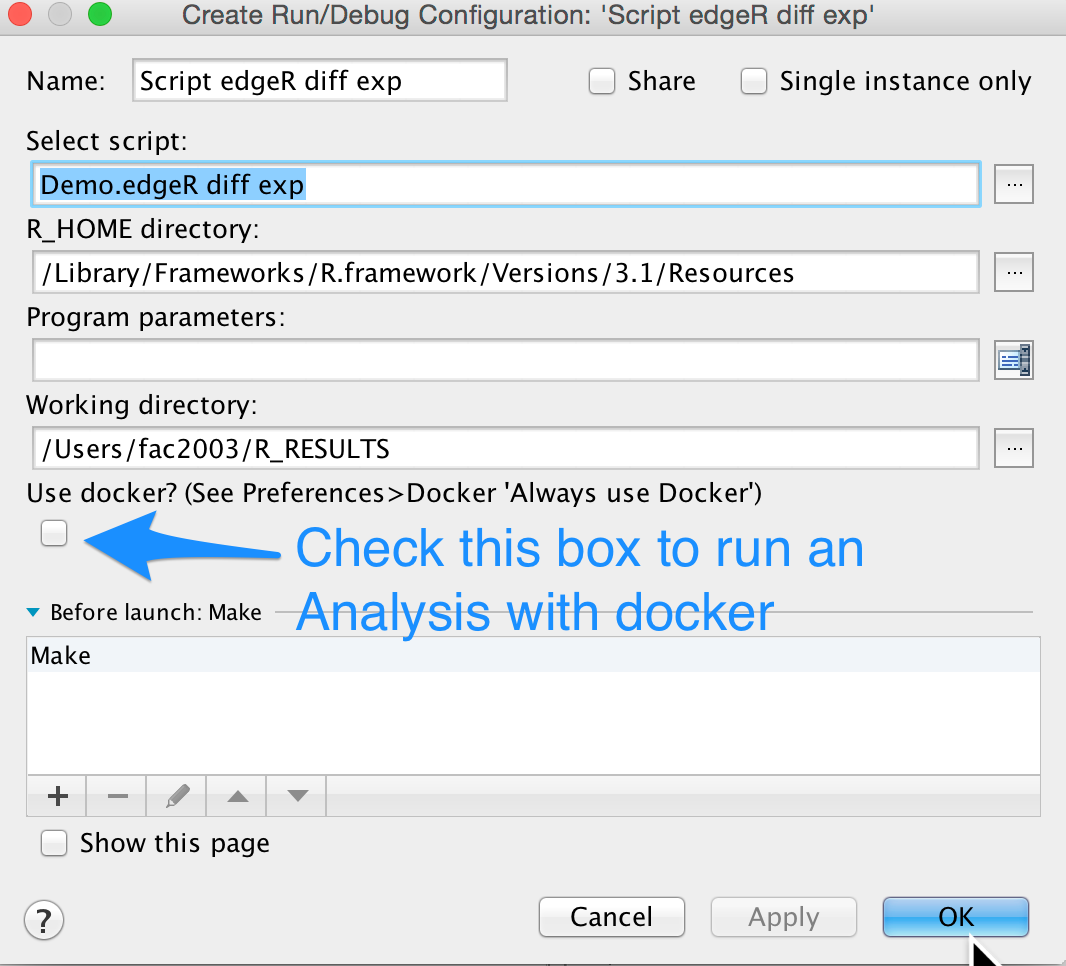
\includegraphics[width=\figWidthNarrow]{figures/CheckThisBoxToRunWithDocker.png}
\caption[Run With Docker.]{\textbf{Run With Docker.} Right-click on an Analysis and do \menu{Create <analysis name>}. You will be presented with the Run Configuration customization dialog. Check the box to run with docker. Disable the check-box to run directly against the R installation on your computer (this behavior was the default prior for MetaR 1.3-).  }
\label{fig:RunWithDocker}
\end{SCfigure}



%	CHAP EdgeR
%----------------------------------------------------------------------------------------

\chapterimage{blue-chapter-head_4-reduced.pdf} % Chapter heading image

\chapter{EdgeR}\label{chap:EdgeR}
The EdgeR language (\texttt{org.campagnelab.metaR.edgeR}) has been developed as a illustration of language composition with MetaR. 
%	CHAP Limma Voom
%----------------------------------------------------------------------------------------

\chapterimage{blue-chapter-head_4-reduced.pdf} % Chapter heading image

\chapter{Limma Voom}\label{chap:LimmaVoom}

\begin{remark}
Limma Voom is a statement introduced in MetaR 1.3.
\end{remark}
\section{Overview}
The Limma Voom statement makes it possible to use the Limma R package and the Limma Voom adjustment to analyze RNA-Seq data with Limma. Similarly to EdgeR, the language that provides the \texttt{Limma Voom} statement must be added to the model where you plan to use the statement in analysis. The name of the language is \textit{org.campagnelab.metar.limma}. Note that this language depends on \textit{org.campagnelab.metar.models}, which should also be imported.


\section{The Limma Voom Statement}
The \texttt{limma voom} statement performs tests of differential expression using read counts contained in a table of data. The statement has the following attributes. Figure~\ref{fig:NewLimmaVoom} presents a newly created Limma Voom statement.
\begin{figure}[h!tbp]
  \centering
  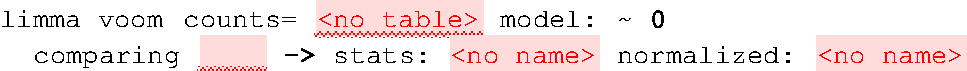
\includegraphics[width=\figWidthWide]{figures/NewLimmaVoom.pdf}
\caption[New Limma Voom Statement.]{\textbf{New Limma Voom Statement.}}
\label{fig:NewLimmaVoom}
\end{figure}
\paragraph{counts table}
The table must contain columns annotated with the ``counts'' group. Bind this table reference to a table that contains non-normalized read counts.

\paragraph{model}
You can use the model attribute to enter a linear model. Limma Voom will use this model to model the mean and variance of the data. You can enter a linear model by typing \texttt{+} followed by the name of a group usage attached to the counts table. Repeat to add multiple factors to the model. 

\paragraph{comparing}
The comparing attribute makes it possible to define the statistics that should be tested for difference with zero. After you have defined a model with several factors (corresponding to group usage), the factor levels (corresponding to group names) will be offered for auto-completion. The factor level name stands for the average of the columns annotated with the group. See Figure~\ref{fig:LimmaVoomExample} for an example. 

\paragraph{normalized}
This attribute holds a table of normalized counts that will be produced when the \texttt{limma voom} statement is executed. You should name the table of normalized counts to make it possible to reference it later. Normalized counts are available even when the model has a single factor (in which case adjust counts would not work because there is no batch to remove).

\paragraph{adjusted counts}
This attribute is exposed under the Inspector Tab(\inspectorTabIcon). It takes a boolean value: either true or false. When true, the limma voom statement will produce a table of adjusted counts. Data in this table is adjusted to remove the effect of covariates described in the model, but not used in the comparing attribute. This is useful to remove the effect of batches, or other cofactors expected to affect expression. Adjusted counts are implemented with the Limma removeBatches function.   
 
\section{Example}
Figure~\ref{fig:LimmaVoomExample} presents an example where the \texttt{Limma Voom} statement configured with a model (one factor: \texttt{LPS}) to call differences between columns labeled with the groups \texttt{LPS=YES} and \texttt{LPS=NO}.



\begin{figure}[h!tbp]
  \centering
  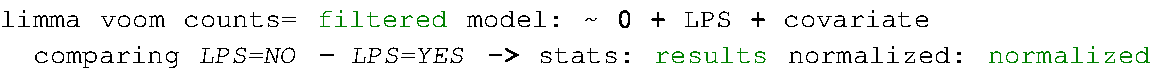
\includegraphics[width=\figWidthWide]{figures/LimmaVoomExample.pdf}
\caption[Limma Voom Example.]{\textbf{Limma Voom Example.}  Since version 1.8, limma voom outputs normalized counts.\index{New in MetaR 1.8}}
\label{fig:LimmaVoomExample}
\end{figure}



%----------------------------------------------------------------------------------------
%	CHAP Sleuth
%----------------------------------------------------------------------------------------

\chapterimage{blue-chapter-head_4-reduced.pdf} % Chapter heading image
\chapter{Sleuth}\label{chap:Sleuth}\index{Sleuth}\index{Kallisto}

\section{Overview}
Sleuth is a package for differential expression testing designed to be used with results obtained with Kallisto~\cite{bray2016near}. In order to use Sleuth, you first need to map RNA-Seq reads with Kallisto against a reference transcriptome. This task can be accomplished with NextflowWorkbench~\cite{kurs2016nextflowworkbench} (we distribute a workflow to perform pseudo-alignments with Kallisto and use this workflow in the NW training sessions). 


When the workflow completes, you will be able to download Kallisto result directories. In this Chapter, we assume that you download and organize Kallisto results under a single directory we will refer to as  \texttt{KALLISTO\_RESULTS}.

\section{Sleuth statement}
The \texttt{Sleuth} statement, alias \texttt{sleuth} is provided in the \textit{org.campagnelab.metar.sleuth} language. Import this language in a model where you want to Sleuth for data analysis.

After downloading Kallisto results, create or open a MetaR analysis and type sleuth. A new statement such as shown in Figure~\ref{fig:NewSleuthStatement} will be created.

\begin{figure}[h!tbp]
  \centering
  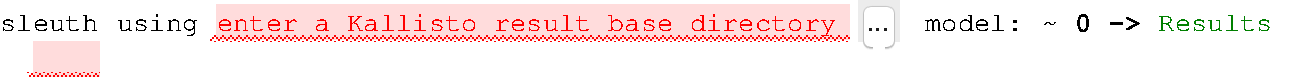
\includegraphics[width=\figWidthWide]{figures/NewSleuthStatement-1.pdf}
\caption[New Sleuth Statement.]{\textbf{New Sleuth Statement.}}
\label{fig:NewSleuthStatement}
\end{figure}

The statement has three attributes:
\paragraph{Kallisto Result Base Directory}
This is a string attribute where you can paste the path to \texttt{KALLISTO\_RESULTS}. Once pasted, if the directory contains Kallisto result sub-directories, the information is organized into a MetaR Table, that will appear in the model. An import statement is added to the analysis and the table becomes referenced by the sleuth statement. A sleuth statement bound to a table is shown in Figure~\ref{fig:KallistoBoundToTable}. At this point, you can annotate the table as you would for a Limma voom or EdgeR analysis: add column groups to columns corresponding to samples and annotate the groups with usages to define factors that you would like to include the analysis (see Chapter~\ref{chap:Tables} to learn how to do this).
For instance, using the Kallisto results from the Sleuth tutorial, the ColumnGroupContainer and Table would look as shown on Figure~\ref{fig:AnnotatedTable}.



\begin{figure}[h!tbp]
\centering
  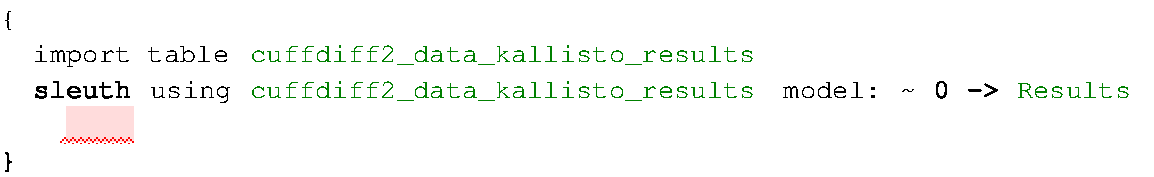
\includegraphics[width=\figWidthWide]{figures/SleuthBoundToTable-1.pdf}
\caption[Sleuth Statement Bound to a Table.]{\textbf{Sleuth Statement Bound to a Table.} The statement shown has been bound to a table by entering a valid Kallisto results directory.}
\label{fig:KallistoBoundToTable}
\end{figure}

\begin{figure}[h!tbp]
  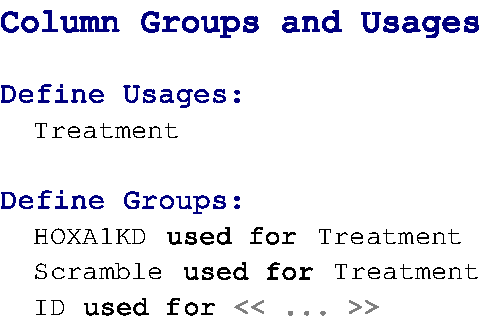
\includegraphics[width=\figWidthTiny]{figures/AnnotatedColumnGroupSleuth-1.pdf}
    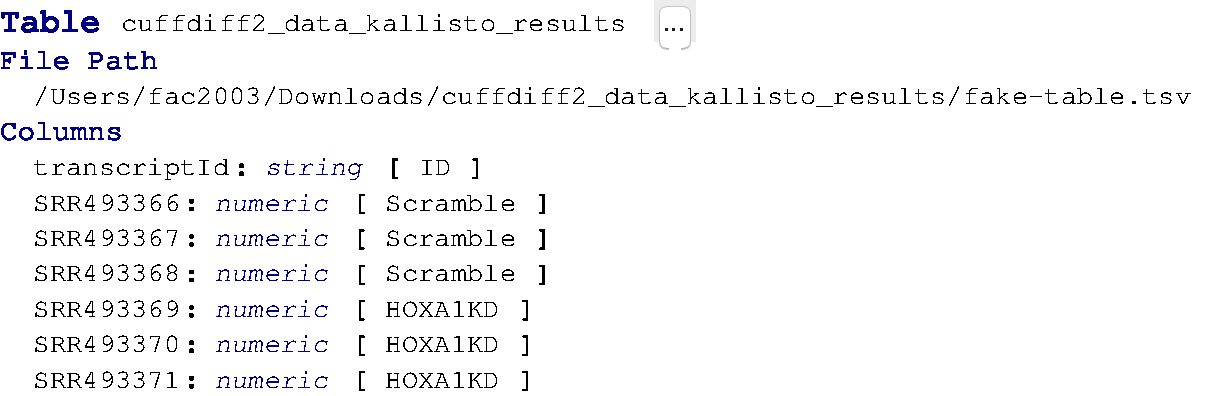
\includegraphics[width=\figWidthWide]{figures/AnnotatedTableSleuth-1.pdf}
\caption[ColumnGroup and Table for Sleuth Tutorial]{\textbf{ColumnGroup and Table for Sleuth Tutorial} Left: ColumnGroupContainer configured for the Sleuth tutorial. Right: Table imported from Kallisto base directory, and annotated with the Scramble and HOXA1KD groups.}
\label{fig:AnnotatedTable}
\end{figure}

\paragraph{Full Model}
A model attribute can be specified after \texttt{model:}. This model should represent the full set of factor/group usages you plan to use to model expression data. You need to annotate columns of the table with groups and group usage before you can use auto-completion to define the model. 

\section{Statistical Test}
The attribute shown on the second line determines the type of statistical test to perform. Sleuth supports two options at this time:
\begin{itemize}
  \item Wald test
  \item Likelihood Ratio Test (LRT)
\end{itemize}

Place the cursor over the pink cell and use auto-completion to choose one of these options. 
\paragraph{Likelihood Ratio Test}\index{LRT}\index{Likelihood Ratio Test}
If you select the LRT, you get to enter a label and a second model. The label is a text string that helps you remember what the alternate model represents. Note that Sleuth only supports an alternate model that is fully contained in the full model. This means that you can remove covariates from the alternate model, but not add some that are not present in the full model (at this time, MetaR does not check for this condition, so watch out). 

\begin{center}

\includegraphics[width=\figWidthNarrow]{figures/SleuthLRT-1.pdf}
\end{center}


\paragraph{Wald Test}\index{Wald Test}

If you select Wald Test, you get the option of entering one group and one usage. The combination should identify a condition for which you are seeking to find differentially expressed transcripts. It is unclear what the test reports when there are several levels to a factor (i.e., a group usage associated with three or more groups).

\begin{center}
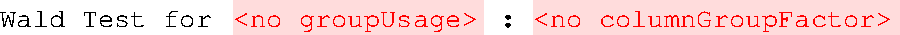
\includegraphics[width=\figWidthNarrow]{figures/SleutWaldTest-1.pdf}
\end{center}

%----------------------------------------------------------------------------------------
%	CHAP Biomart
%----------------------------------------------------------------------------------------

\chapterimage{blue-chapter-head_4-reduced.pdf} % Chapter heading image
\chapter{Biomart}\label{chap:Biomart}
%upload images for examples
%invert description and itemize statement

% introduction
\section{Overview}
The BioMart project develops software and data services that are made available to the international scientific community. Users of MetaR can access data Marts provided by BioMart, providing access to a wide range of research data . Similarly to EdgeR and Limma, BioMart support is provided in a MetaR language extension. This means that in order to access BioMart with MetaR, you first need to add the Biomart language to the model where you create the analysis. To do so, you can press~\keys{\ctrl+L} and add language \textit{org\allowbreak.campagnelab\allowbreak.metar\allowbreak.biomart}. After adding the biomart language to the model, you can create \texttt{query biomart} statements, described in the following sections. 

\section{The Biomart Statement}
The \texttt{query biomart} statement makes it possible to interactively specify which data should be retrieved from a mart (using attributes and filters). Data downloaded from Biomart will be stored in a new table. Figure~\ref{fig:NewBiomart} presents a newly created Biomart statement.
The \texttt{query biomart} statement has the following parameters.
\begin{itemize}
\item database
\item dataset
\item attributes
\item filters
\end{itemize} 

 \begin{figure}[h!tbp]
  \centering
  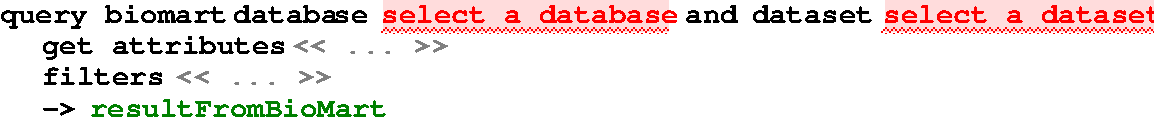
\includegraphics[width=\figWidthWide]{figures/NewBiomart.pdf}
\caption[New Query Biomart Statement.]{\textbf{New Query Biomart Statement.}}
\label{fig:NewBiomart}
\end{figure}


\paragraph{database}
The first time you will create the \texttt{query biomart} statement, you will automatically download the available Biomart databases. To choose one of them, go to the text \textit{select a database}. Then, press \keys{\ctrl+\space} to display all available databases. Select one of them by pressing \keys{\return}. 


 \paragraph{dataset} 
Once a database is selected, you need to choose a dataset. To choose one, press \keys{\ctrl+\space} to display all available datasets, on the text \textit{select a dataset}. Then, press \keys{\return}, to select your dataset. \newline
A dataset as two childrens:
\begin{itemize}
\item attributes, which will be the columns of your result table.
\item filters, which allow you to restrict your result table for some criteria.
\end{itemize}
\begin{remark}
Sometimes, a dataset cannot be associated with attributes or filters. In this case, in the auto completion menu for both attributes and filters will display the message \textit{"No available filter or attributes in this dataset"}. The selected dataset is no more available in Biomart. You must change your dataset or database. 
\end{remark}

\paragraph{attributes}
Attributes are columns of your result table. Figure~\ref{fig:attributeBiomart} presents a new biomart attribute. An attribute has three parameters:
\begin{itemize}
\item attribute, a column you want to retrieve on your result table. Press \keys{\ctrl+\space} to display the available column.
\item type, of  the attribute rows values. It exist three  types
boolean, numeric and string (\textit{ by default}). To change the type, press \keys{\ctrl+\space}.
\item column group, an attribute can have a group such as "ID". The user can display the autocompletion menu by pressing \keys{\ctrl+\space}. Group must be defined in the Column Group Container to be added to the result table.
\end{itemize}

\begin{remark}
You must select at least one column to run your query biomart Statement.
\end{remark}

 \begin{figure}[h!tbp]
  \centering
  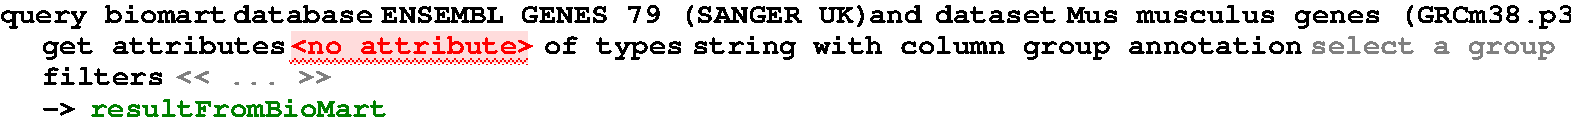
\includegraphics[width=\figWidthWide]{figures/BiomartAttribute.pdf}
\caption[Select an attribute in a biomart dataset.]{\textbf{Select an attribute in a biomart dataset.} An attribute contains any information you want to retrieve on your result table. It has a name, a type and a column group annotation. Attributes are related to a specific dataset.}
\label{fig:attributeBiomart}
\end{figure}
\paragraph{Filters}
Filters allow you to restrict your result for some criteria. this criteria are link directly to your dataset. Figure~\ref{fig:BiomartFilter} presents a new biomart filter. It exist four filter categories: 
\begin{itemize}
\item boolean, you want to retrieve or excluded only data which have an information. \textit{For example, if this gene has or has not a Mirbase ID.}
\item text, you have to enter a text in this area. the query will return only informations which match your text. \textit{For example  a specific GO term.}
\item list,  you need to choose a value from a define list. \textit{For example a specific chromosome in a specie.}
\item id list, you can restrict your results from a set of ids. This ids can come from a set of ids define before the statement, or directly from an annotated table with an (ID group).  
\end{itemize}

 \begin{figure}[h!tbp]
  \centering
  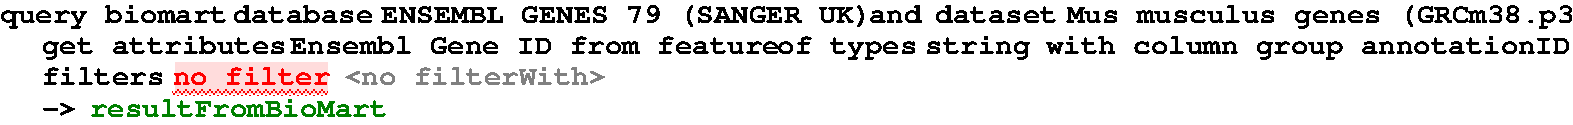
\includegraphics[width=\figWidthWide]{figures/BiomartFilter.pdf}
\caption[New Biomart Filter]{\textbf{New Biomart Filter.} A filter allow you to apply constraints to you results. It exist four filters categories: boolean, text, list and id list. Filters are related to a specific dataset.}
\label{fig:BiomartFilter}
\end{figure}

\paragraph{table}
The future table where your result will be stored. Column annotation is display under the Inspector Tab (\inspectorTabIcon).
\section{Examples}
\subsection{Example 1}
Figure~\ref{fig:BiomartExample1} show how to obtain a table from the Ensembl database and Human dataset. The result table "resultFromBiomart" contains 2 columns, the Ensembl Gene and Exon ID, where the first column is annotated as a group "ID". This result are filters from a list of gene and which do not contains a Mirbase ID.
 \begin{figure}[h!tbp]
  \centering
  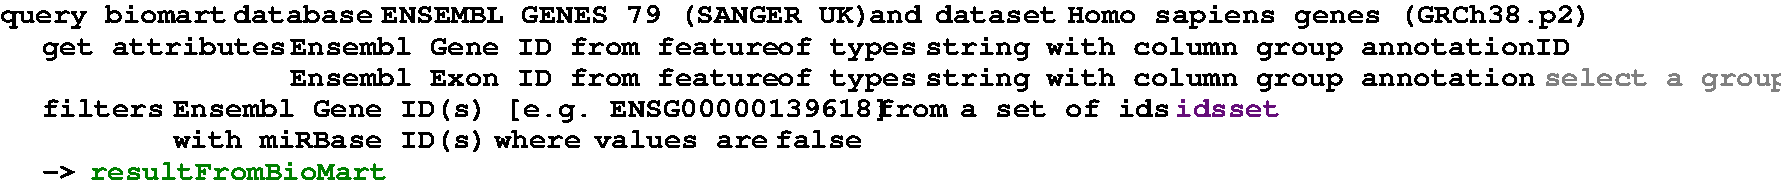
\includegraphics[width=\figWidthWide]{figures/BiomartExample1.pdf}
\caption[Biomart Example 1]{\textbf{ Biomart Example 1.}}
\label{fig:BiomartExample1}
\end{figure}

\subsection{Example 2}
Figure~\ref{fig:BiomartExample2} show how to obtain a table from the Paramecium bibliography. The result table "resultFromBiomart" contains 2 columns, the PubMed ID and the abstract, where the publication year is upper 2000.
 \begin{figure}[h!tbp]
  \centering
  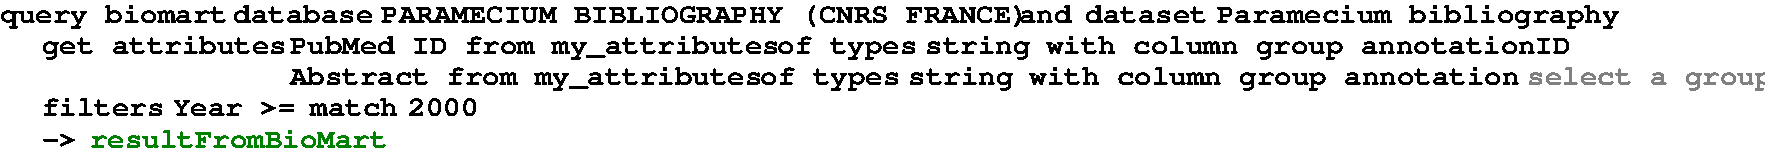
\includegraphics[width=\figWidthWide]{figures/BiomartExample2.pdf}
\caption[Biomart Example 2]{\textbf{ Biomart Example 2.}}
\label{fig:BiomartExample2}
\end{figure}


%----------------------------------------------------------------------------------------
%	CHAP Functions
%----------------------------------------------------------------------------------------

\chapterimage{blue-chapter-head_4-reduced.pdf} % Chapter heading image

\chapter{R Functions}\label{chap:RFunctions}\index{Functions}\index{R Functions}

\section{Overview}
Since version 1.4, MetaR supports calling R functions directly. This Chapter describes how you can use this feature to take advantage of the many functions available in R packages to transform data in your MetaR Analyses. 

\subsection{Function w}
Function stubs\index{Function stubs} are provided that represent functions offered by different packages. Stubs do not provide the code associated with the function, but describe the function name and the arguments of the function and its default values. This information is used to support auto-completion for R functions. 

We provide pre-imported stubs for the packages used during the MetaR training sessions, namely: \textit{base}, \textit{graphics}, \textit{data.table}, \textit{pheatmap}, \textit{biomaRt}, \textit{edgeR} and \textit{limma}. While stubs are provided, they are not immediately available in a MetaR analysis. In order to use R function stubs, you need to 
\begin{itemize}
  \item Add \textit{org.campagnelab.R} to the list of Used languages in the model where you need the stubs.
  \item Use the \texttt{import stubs} statement followed with the name of the package that provides the functions that you wish to use.
\end{itemize}

\noindent{}For instance, if you enter the following statement: 
\begin{lstlisting}
import stubs base
\end{lstlisting}

\noindent{}After typing this statement, the \textit{base} package R functions will become available inside the Analysis where you imported these stubs. You can use R function using the \texttt{eval} statement or expression (see Sections~\ref{sec:EvalStatement}and \ref{sec:EvalExpression}).

If you need a package that is not yet provided with MetaR, you should use the \texttt{import package} statement (see Section~\ref{sec:ImportPackageStatement}). 

\section{Import Stubs Statement}\label{sec:ImportStubsStatement}\index{Import function stubs}
The \texttt{import stubs} statement (alias import stubs) makes it possible to import functions in packaged already packaged with MetaR. Simply type import stubs, and use auto-completion to locate the package for which you need to import function stubs.


\section{Import Package Statement}\label{sec:ImportPackageStatement}\index{Import package}

The \texttt{import package} statement (alias import package) makes it possible to import functions in any R package. If the package is already provided in MetaR, the \texttt{import package} statement  will be automatically replaced with the equivalent \texttt{import stubs} statement (see Section~\ref{sec:ImportStubsStatement}). Figure~\ref{fig:NewImportPackage} presents an import package statement. 
\paragraph{name} The name attribute is a string and must be the name of an R package, suitable to install the package in R with  \texttt{install.packages("name")}.

\begin{figure}[h!tbp]
  \centering
  
\includegraphics[width=\figWidthSmall]{figures/NewImportPackage.pdf}
\caption[New Import Package Statement.]{\textbf{New Import Package Statement.}  Enter the name of an R package to import this package into the Analysis. Note that the package will be visible only after you run the Analysis at least once.}
\label{fig:NewImportPackage}
\end{figure}

\begin{remark}
If you need to import a Bioconductor package, use the \texttt{import bioconductor package} statement instead.
\end{remark}
After you execute the Analysis that contains the import package statement, the package will be installed in the version of R that you are using, if needed and the package loaded. 
Use the ``Reload Functions and Create Stubs'' intention after you have executed the statement to create the Stubs root node for the functions in the package. When you call this intention, the package will be inspected for function declarations, and these declarations will be written to a \texttt{Stubs} root node in the model where the \texttt{Analysis} is located. Following this process, the \texttt{import package} statement is replaced with the import stubs statement, loading the stubs directly from the model. Note that you can inspect the stubs object to learn about the functions available in the package represented by the stubs. 


\section{Import Bioconductor Package Statement}\label{sec:ImportBioconductorPackageStatement}\index{Import bioconductor package}\index{Bioconductor}
Importing a bioconductor package is very similar to importing a regular R package, but you need to use the \texttt{import bioconductor package} statement. This statement ensure appropriate installation and loading of bioconductor packages in R. Figure~\ref{fig:NewBioconductorImportPackage} presents a new \texttt{import bioconductor package} statement.

\begin{figure}[h!tbp]
  \centering
  
\includegraphics[width=\figWidthNarrow]{figures/NewImportBioconductorPackage.pdf}
\caption[New Import Bioconductor Package Statement.]{\textbf{New Bioconductor Import Package Statement.}  Enter the name of an Bioconductor package to import this package into the Analysis. Note that the package will be visible only after you run the Analysis at least once.}
\label{fig:NewBioconductorImportPackage}
\end{figure}

\section{Stubs}\index{Stubs}\label{sec:Stubs}
Stubs represent functions from R regular or bioconductor packages. We do not recommend creating Stubs manually. The easiest way to create Stub root nodes is by using the \texttt{import package} and \texttt{import bioconductor package} statements. Figure~\ref{fig:StubsExample} presents a snapshot showing a few functions located in the base Stubs root node (R version 3.1.3).
\begin{remark}
Stubs distributed with MetaR are packaged in models named after the version of R which provided the package, in an effort to help track differences between major R versions.
\end{remark}


\begin{figure}[h!tbp]
  \centering
  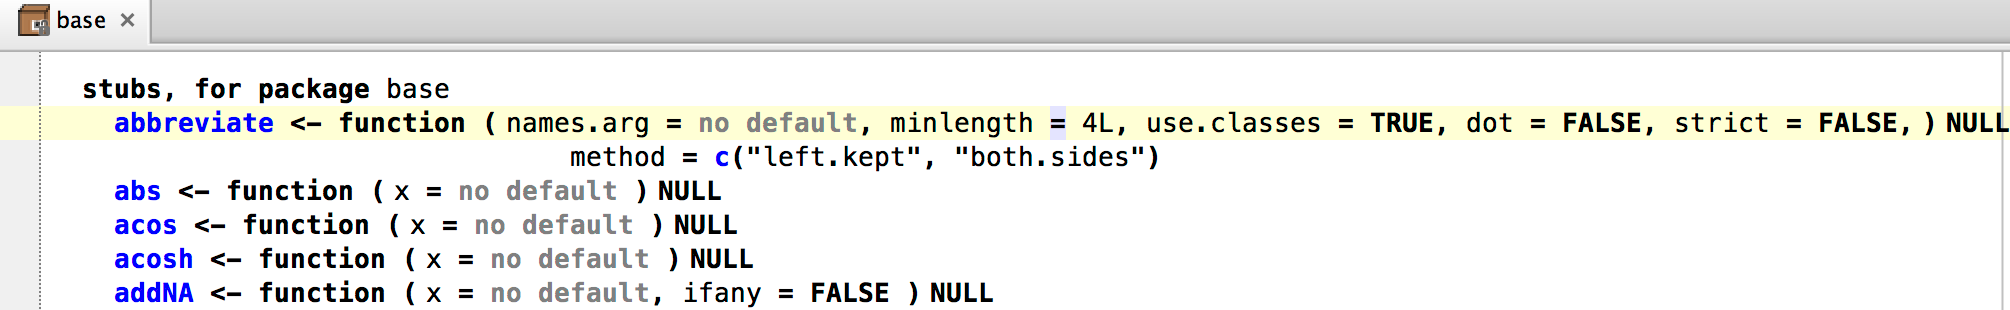
\includegraphics[width=\figWidthWide]{figures/BaseStubsSnapshot.png}
\caption[Base Package Stubs Illustration.]{\textbf{Base Package Stubs Illustration.}  This snapshot presents the beginning of the stubs base root node, located in model \texttt{R3\_1\_3} (language \textit{org\allowbreak{}.campagnelab\allowbreak{}.metar\allowbreak{}.r\allowbreak{}.stubs}).}
\label{fig:StubsExample}
\end{figure}

\section{Eval Statement}\label{sec:EvalStatement}
The \texttt{eval} statement can be used to call R functions that produce some side-effect. When you import the devkit \textit{org.campagnelab.R} into a model, you can type \texttt{eval} in an Analysis node as a statement. The statement will offer auto-completion for function names imported into the analysis. If you do not see the function that you would like to use, make sure you have imported the stubs for the package that contains this function. When you run the analysis, the function named after \texttt{eval} will be executed. Note that you cannot retrieve a return value with the \texttt{eval} statement. You must use the \texttt{eval} expression to obtain a value. The eval statement is useful when you need to call a function that has a side-effect, for instance the setkey function of data.table.

\section{Eval Expression}\label{sec:EvalExpression}
The \texttt{eval} expression can be used to call R functions inside a MetaR expression. MetaR expressions are used in the \texttt{subset} statement, and in some plotting statements (e.g., \texttt{boxplot} or \texttt{histogram}).  When you import the devkit \textit{org.campagnelab.R} into a model, you can type \texttt{eval} inside an expression. The \texttt{eval} expression will offer auto-completion for function names imported into the analysis. If you do not see the function that you would like to use, make sure you have imported the stubs for the package that contains this function. 


\section{Accessing MetaR Columns within R Expressions}\label{sec:AccessingMetaRColumns}\index{Accessing MetaR columns within R expressions}
When you use either the eval statement or expression, you will often need to access columns from a MetaR table to pass as arguments to the function. You can do this with the \texttt{\$} node, which bridges between R expressions (used inside R functions) and MetaR columns. After typing \texttt{\$}, the node will auto-complete to the set of columns visible at this point of the MetaR \texttt{Analysis}. 


\section{Example}
Figure~\ref{fig:TestinFunctionsExample} presents an example where stubs are imported for packages pre-packaged with MetaR and the import package statement is used to import grDevices.
\begin{figure}[h!tbp]
  \centering
  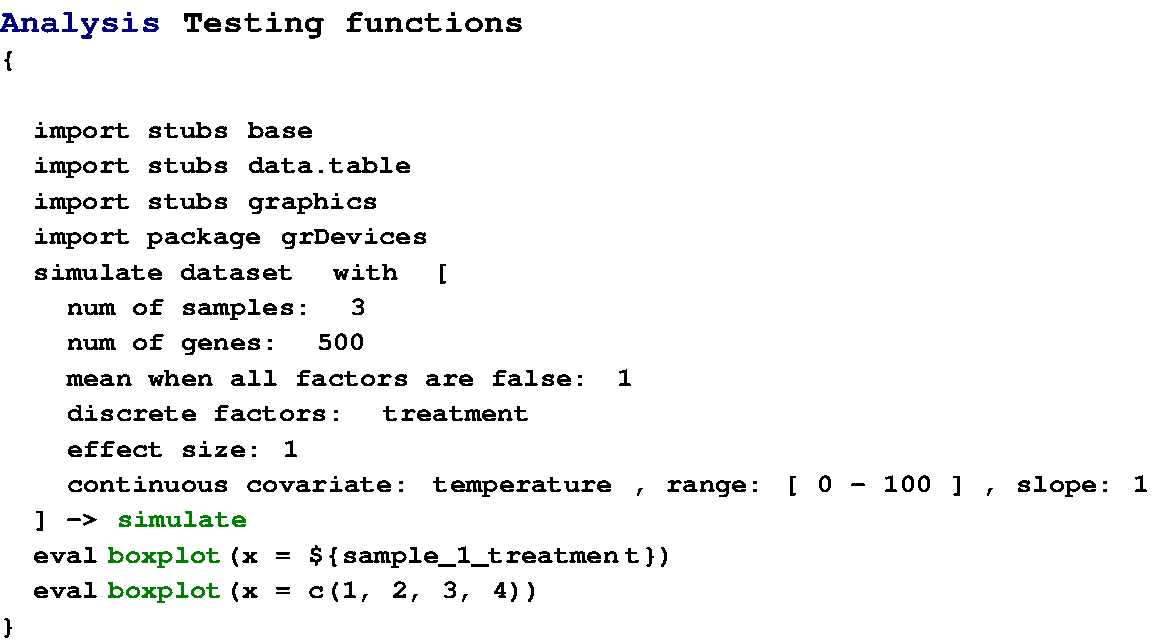
\includegraphics[width=\figWidthWide]{figures/TestinFunctionsExample.pdf}
\caption[Functions Example.]{\textbf{Functions Example.} This example imports stubs and one package, creates a table with three columns (see Simulate statement in Chapter~\ref{chap:SimulatingDatasets}) and evaluates two R functions. The first use of the \texttt{boxplot} function plots the values of the column \texttt{sample\_1\_treatment} that was generated with the simulate statement. The second call to \texttt{boxplot} is given a list of four integers.}
\label{fig:TestinFunctionsExample}
\end{figure}


%	CHAP Simulate Datasets%----------------------------------------------------------------------------------------

\chapterimage{blue-chapter-head_4-reduced.pdf} % Chapter heading image

\chapter{Simulating Datasets}\label{chap:SimulatingDatasets}

\section{Why simulating datasets}

To test or validate an Analysis script with large datasets it is sometimes useful to create a simulation of such datasets when they are not available. This approach could be also beneficial at experimental design time to validate certain assumptions before running (expensive) experiments.

MetaR is extended with a Simulate Dataset command that allows to create datasets starting from a few parameters. In order to use the command, the Simulation language (\texttt{org.campagnelab.metaR.simulation}) has to be imported in the current model (use \keys{\cmd+L} and select the language from the list). Figure~\ref{fig:NewSimulateStatement} shows a new Simulate Dataset statement.

\begin{figure}[h!tbp]
  \centering
  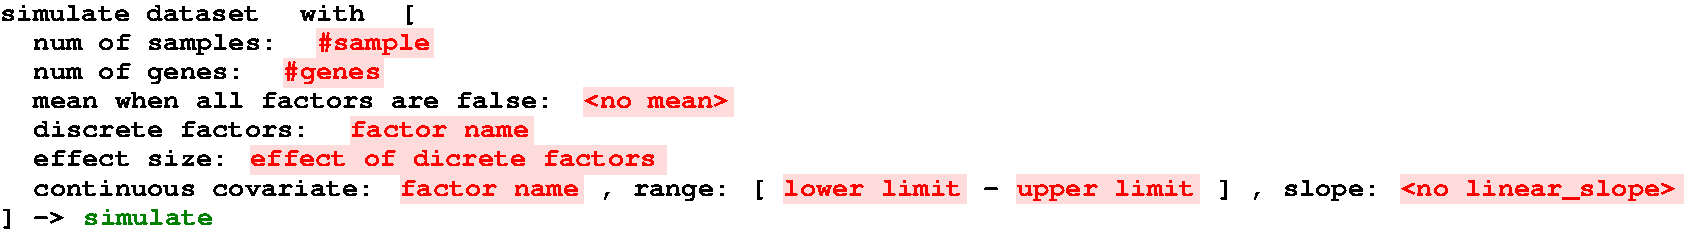
\includegraphics[width=\figWidthWide]{figures/NewSimulateStatement.pdf}
\caption[New Simulate Dataset Statement.]{\textbf{New Simulate Dataset Statement.} A new Simulate Dataset statement created after you have added the \texttt{org.campagnelab.metaR.simulation} language to the model's MPS Used Languages.}
\label{fig:NewSimulateStatement}
\end{figure}
 

\section{The Simulate Dataset Statement}
The Simulate Dataset statement is highly configurable and lets you create a variety of datasets for different needs.  

\paragraph{num of samples}
The number of samples in the dataset. Each sample is named according to the results of the simulation. If the simulation decides that the sample name \emph{sample\_3 }has been treated with a discrete factor named \emph{LPS}, it is renamed to \emph{sample\_3\_LPS} to make it easy to identify the affection.

\paragraph{num of genes}
The number of genes in the dataset. Each gene is renamed according to the results  of the simulation. If the simulation decides that the gene named \emph{gene\_2} is affected by a discrete factor named \emph{LPS}, it is renamed to \emph{gene\_2\_LPS} to make it easy to identify the treatment.

\paragraph{mean}
...

\paragraph{discrete factors}
List of treatments used in the simulation. About 50\% of the samples will be considered treated with each factor specified here. About 30\% of the genes will be considered affected by each factor.

\paragraph{effect of discrete factors}
The impact of each discrete factor on the data generated by the simulation

\paragraph{continuous covariate}
...


\section{Example}

\begin{figure}[h!tbp]
  \centering
  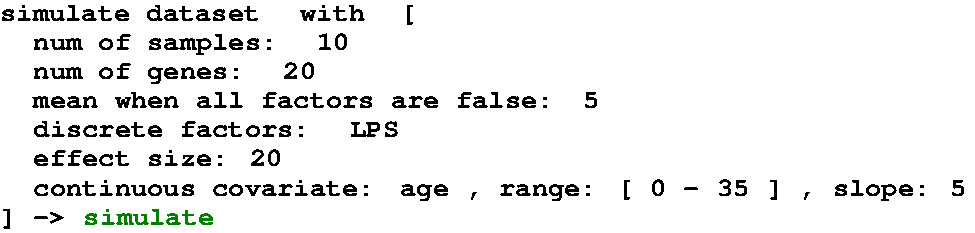
\includegraphics[width=\figWidthWide]{figures/SimulateStatementWithParameters.pdf}
\caption[SimulateDataset Example.]{\textbf{Simulate Dataset Example.} The statement will create a dataset with a single discrete factor (LPS) and a covariate factor (age) with a range of 0 to 36 (for instance, this could be the mice age in a mouse model). }
\label{fig:SimulateDatasetExample}
\end{figure}


\begin{figure}[h!tbp]
  \centering
  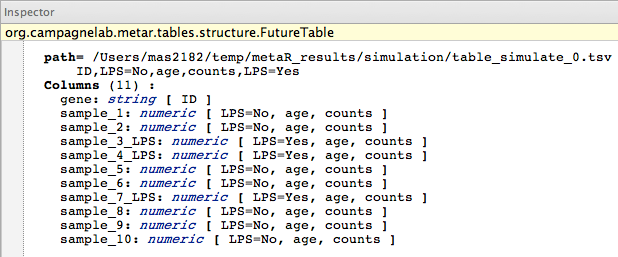
\includegraphics[width=\figWidthWide]{figures/SimulateTableInspector.png}
\caption[SimulateDataset Inspector.]{\textbf{Preview of the Dataset structure as shown in the Inspector.}}
\label{fig:SimulateDatasetInspector}
\end{figure}


\begin{figure}[h!tbp]
  \centering
  \includegraphics[width=\figWidthNarrow]{figures/SimulateCovariateTableInspector.png}
\caption[SimulateCovariateTableInspector.]{\textbf{Covariate Table generated with Simulate Dataset.}}
\label{fig:SimulateCovariateTableInspector}
\end{figure}


\begin{figure}[h!tbp]
  \centering
  \includegraphics[width=\figWidthWide]{figures/SimulateTableViewer.png}
\caption[Table generated with Simulate Dataset.]{\textbf{Table generated with Simulate Dataset (partial view).}}
\label{fig:SimulateDatasetViewer}
\end{figure}



%----------------------------------------------------------------------------------------
%	CHAP introduction
%----------------------------------------------------------------------------------------

\chapterimage{blue-chapter-head_4-reduced.pdf} % Chapter heading image

\chapter{Extending MetaR}\label{chap:ExtendingMetaR}

\section{Overview}
Because MetaR is developed in the MPS language workbench, you can use language composition as a way to extend the MetaR language. In this Chapter, we provide a very simple example to illustrate how to extend MetaR through language composition. 

Let's assume that you have just learned about the \texttt{heatmap.2} function provided in the \texttt{gplots} R package. You wish to use this function to create heatmaps with MetaR. To achieve this, you would follow the following steps: 
\begin{enumerate}
\item Create a new MPS Language.
  \item Create a \texttt{Heatmap.2} language concept in the Structure Aspect of the language (see~\cite{campagne2014mps}).
  \item Customize the Generator to transform instances of the \texttt{Heatmap.2} into R code.
\end{enumerate}

\section{Create a new Language}
Let's create a new language. To do this, select the project and do \menu{right-click>New>Language}. Name the language something like \texttt{your.domain.\allowbreak{}heatmap}.When the language has been created, select its name under the Project Tab and adjust Dependencies to include \textit{org.campagnelab.metaR.tables}. Set the Scope to Extend (this will allow statements of this new language to extend concepts of \textit{org.campagnelab.metaR.tables}). 

\section{Create a new Language Concept}
Select the Structure Aspect of the \textit{your.domain.\allowbreak{}heatmap} language and do \menu{right-click>New >Concept}. Name the concept \texttt{Heatmap2}. Define the extends clause to be \texttt{Statement} (from language \textit{org.campagnelab.metar.tables}). The resulting concept should appear as shown in Figure~\ref{fig:Heatmap2Concept}.

\paragraph{concept alias}
Define the alias of the concept. Use \texttt{heatmap2}. An instance of the concept will be created when you type this keyword in the editor. 

\paragraph{reference to a table}
To plot a heatmap, we will take data from a MetaR table. This can be achieved by adding a TableRef child to the \texttt{Heatmap2} concept.
\paragraph{heatmap produces a plot}
The heatmap2 statement will produce a plot, so you need to add a child of type \texttt{Plot}. You may call this child `plot' for simplicity.

\begin{figure}[htbp]
  \centering
  \includegraphics[width=\figWidthNarrow]{figures/Heatmap2Concept.pdf}
\caption[Heatmap2 Concept.]{\textbf{Heatmap2 Concept.} The Heatmap2 concept extends Statement. When the language is composed with MetaR, Heatmap2 will become available for auto-completion whenever a MetaR Statement can be used.}
\label{fig:Heatmap2Concept}
\end{figure}

\section{Define the Editor}
An MPS editor customizes how a node appears in the editor. Create an editor for \texttt{Heatmap2} (see~\cite{campagne2014mps}) and define its content as shown in Figure~\ref{fig:EditorForHeatmap2}.
\begin{SCfigure}
  \centering
  \includegraphics[width=\figWidthNarrow]{figures/EditorForHeatmap2.pdf}
\caption[Editor of the Heatmap2 Statement.]{\textbf{Editor of the Heatmap2 Statement.} Notice how the editor simply shows the name of the statement, delegates to the TableRef editor to render the table reference, and delegates to the Plot editor to show the plot child.}
\label{fig:EditorForHeatmap2}
\end{SCfigure}

\section{Generate R Code}
In order to generate the statement to R code, we will use the MPS Generator aspect. 

In the first step, we create a reduction rule, see Figure~\ref{fig:GeneratorHowToStep1} and~\cite{campagne2014mps} (Generator Aspect chapter). The rule indicates that nodes of the \texttt{Heatmap2} concept will be transformed with the \texttt{reduce\_Heatmap2} template. The template was created using the \textbf{New Template} intention found on the reduction rule node. See detailed instructions in~\cite{campagne2014mps}.

\begin{figure}[h!tbp]
  \centering
  \includegraphics[width=\figWidthWide]{figures/GeneratorHowToStep1.png}
\caption[Generate R Code: Step 1.]{\textbf{Generate R Code: Step 1.} Start by adding a reduction rule.}
\label{fig:GeneratorHowToStep1}
\end{figure}

The simplest template we can build for the \texttt{Heatmap2} concept is shown on Figure~\ref{fig:SimplestTemplate}. Simply calling the heatmap.2 function is a good start, but trying to run this will fail because the function is not part of a plain R distribution. The next section explains how to install the gplot R package which provides the function and activate it. 

\begin{figure}[h!tbp]
  \centering
  \includegraphics[width=\figWidthWide]{figures/SimplestTemplate.png}
\caption[Simplest template.]{\textbf{Simplest template.} The template simply converts any node of the \texttt{Heatmap2} concept to a line of R code that calls the \texttt{heatmap.2} function with the table as an argument. Notice the use of a property macro to obtain the R name of the table variable from the node table attribute. Open the \inspectorTabIcon{} to see what value the macro will take when a node is generated to R code.}
\label{fig:SimplestTemplate}
\end{figure}

\subsection{Adding package and library support}
MetaR makes it easy to install R packages as they are needed by an analysis. For this to work, we need to declare that the \texttt{Heatmap2} concept depends on the \textit{gplots} R package.  We can do this by adding overriding the default Statement behavior method called \texttt{dependencies()}. This method must return a list of package names that must be installed and loaded before the statement can execute. To override the method, navigate to the Heatmap2 concept in the editor, select the behavior tab, create the behavior and when the empty behavior is shown, select Override Behavior Method (see Figure~\ref{fig:CreateBehaviorAndOverride}).
Replace the body of the method with 
\begin{lstlisting}
return new singleton<string>("gplots");
\end{lstlisting}
Figure~\ref{fig:dependenciesMethodComplete} shows the complete  method. Rebuild the language, then the solution. When you run the Analysis, you will see that the gplots package is being installed:
\begin{lstlisting}
...
Loading required package: gplots
Installing package into '/Users/fac2003/.metaRlibs'
(as 'lib' is unspecified)
also installing the dependencies 'bitops', 'gtools', 'gdata', 
    'caTools'

trying URL ....
\end{lstlisting}

\begin{SCfigure}
  \centering
  \includegraphics[width=\figWidthNarrow]{figures/CreateBehaviorAndOverride.png}
\caption[Override Behavior Methods.]{\textbf{Override Behavior Methods.} When the override dialog appear, choose dependencies() and click OK.}
\label{fig:CreateBehaviorAndOverride}
\end{SCfigure}


\begin{SCfigure}
  \centering
  \includegraphics[width=\figWidthSmall]{figures/dependenciesMethodComplete.png}
\caption[Complete Dependencies Behavior Method.]{\textbf{Complete Dependencies Behavior Method.}}
\label{fig:dependenciesMethodComplete}
\end{SCfigure}

\subsection{Adjust Generator Priorities}
Adjust the generator priorities as shown in Figure~\ref{fig:Generator_Properties_your_domain_heatmap2}. You set priorities, you need to define a Design dependency on \textit{org.campagnelab.metar.tables} in the generator aspect Module Properties dialog. 

\begin{figure}[h!tbp]
  \centering
  \includegraphics[width=\figWidthWide]{figures/Generator_Properties_your_domain_heatmap2.png}
\caption[Adjust Generator Priorities.]{\textbf{Adjust Generator Priorities.} Generation of the Heatmap2 concept need to happen in the same generation phase as the generation of the  \textit{org.campagnelab.metar.tables} concepts. Failure to adjust priorities may result in table names not being correctly inserted in the \texttt{heatmap.2} function call.}
\label{fig:Generator_Properties_your_domain_heatmap2}
\end{figure}

\subsection{Redirecting the plot output}
The next problem with the simple template is that it fails to write the image of the plot in  location where MetaR can find it. This is needed to display the plot preview, or to make it possible to use plots with the \texttt{multiplot} statement.
The strategy we use to handle both cases is to wrap the actual ploting code inside a \texttt{plot\_xxx} function. The function is named with the id of the statement that generates the plot, so that we can easily refer to it in other places where the plot should be reused. We start by defining this function:

\begin{lstlisting}
plot_ $[id]=function(t){                        
  heatmap.2(as.matrix(t)) 
}                                             
\end{lstlisting}

The function accepts one argument: the name of the table to plot. 

\begin{remark}
The number of arguments is up to you, since you will generate both the function and the function calls.

\end{remark}

The next step is to plot to a png file to show a preview of the plot in the inspector. To this end, we redirect the plot output with png(), call the plot function, and close the graphics output (dev.off()):

\begin{lstlisting}
png(file=" $[plot.png]", width= $[w], height= $[h])
plot_ $id( $[table])                           
ignore <- dev.off()                          
\end{lstlisting}
Notice how the parameters of the png function are taken from the Plot node.
For instance, the \texttt{\$[plot.png]} macro will expand to 

\begin{lstlisting}
new RPath(node.plot.getPath()).toString();
\end{lstlisting}


\subsection{Handling errors}
Accurate error reporting is important to the end-user. when things do not go well and the R code fails, it is useful to know precisely which MetaR statement generated the error. In MetaR, this is done by taking advantage of the tryCatch R functions (see \url{http://mazamascience.com/WorkingWithData/?p=912}. 

Because \texttt{tryCatch} is not particularly intuitive and is rather verbose, MetaR extends the \textit{org.campagnelab.TextOutput} language with the \texttt{tryForNode} statement. The tryForNode statement attempts to execute some lines of R code, and reports any errors that occur in these lines with a link to the statement that produced the error or warning. The \texttt{tryForNode} statement is also responsible for showing the \texttt{STATEMENT\_EXECUTED/8289224569309332962/} lines in the Run tool, which are hyperlinked to statements in the editor. 

The statement tryForNode takes an ID, which is the result of the id() method defined for each MetaR statement. The value of the ID can be set as usual with a property macro (its value should be \texttt{node.id()}). Figure~\ref{fig:Heatmap2GeneratorComplete} shows the completed template for Heatmap2. While the statement only needs to call the \texttt{heatmap.2} function, handling possible errors and producing plots that can be reused to build multi-panel figures has added quite a few lines to the output.

\begin{figure}[h!tbp]
  \centering
  \includegraphics[width=\figWidthWide]{figures/Heatmap2GeneratorComplete.png}
\caption[Complete Generator for Heatmap2.]{\textbf{Complete Generator for Heatmap2.} This template wraps the heatmap.2 function call inside a plot function (needed when building figures with multiple panels) and inside a tryFoNode statement. The tryForNode statement generates to the tryCatch R language construct and appropriately reports errors to the end-user.}
\label{fig:Heatmap2GeneratorComplete}
\end{figure}

 
\begin{figure}[h!tbp]
  \centering
  \includegraphics[width=\figWidthWide]{figures/Heatmap2_Execution.png}
\caption[Heatmap2 Execution.]{\textbf{Heatmap2 Execution.} This figure presents an Analysis using the new heatmap2 concept and shows the resulting plot preview in the inspector (bottom right). Error handling and progress indicators can be seen on the bottom left.}
\label{fig:Heatmap2_Execution}
\end{figure}


%----------------------------------------------------------------------------------------
%	CHAP Composable R
%----------------------------------------------------------------------------------------

\chapterimage{blue-chapter-head_4-reduced.pdf} % Chapter heading image

\chapter{Composable R}\label{chap:ComposableR}\index{Composable R}\index{R Language}
\section{Overview}
MetaR release 1.5 was the first release to offer a composable R language for MPS (this language is called \textit{org.campagnelab.metaR.R} in MPS, but also simply referred to as ``composable R'', or \textit{compR}). This Chapter explains how to take advantage of this language, what the advantages of a composable R language are, but also describes the current limitations of its implementation.

\subsection{Advantages}
\paragraph{Composable R supports the full R grammar}

The composable R language implemented in MetaR 1.5+ supports  the equivalent of the R language grammar. 
\begin{remark}
We have developed composable R starting with the ANTRL4 R grammar obtained from \url{https://github.com/antlr/grammars-v4/tree/master/r}. 
\end{remark}
Because this language is composable, you can design micro-languages to compose with R. An example of micro-language composition, to use the biomart statement described in Chapter~\ref{chap:Biomart}, is shown in Figure~\ref{fig:ExampleRunningComposableRLanguageInMPS}.

\begin{figure}[h!tbp]
  \centering
  \includegraphics[width=\figWidthWide]{figures/ExampleRunningComposableRLanguageInMPS.png}
\caption[Example of Micro-Language Composition with Composable R.]{\textbf{Example of Micro-Language Composition with Composable R.} In this example, we have composed the MetaR query biomart statement (see Chapter~\ref{chap:Biomart} with the R language).}
\label{fig:ExampleRunningComposableRLanguageInMPS}
\end{figure}


\paragraph{Fluent editing}\index{Fluent editing}

Composable R supports Fluent Editing\footnote{To learn how to implement this feature for your own languages, see~\cite{campagne2015mps}}. We have designed this technique to make it easier to paste an R code fragment from text into an R script. The technique is also very useful to enter complicated R expressions more quickly than possible with the MPS  projectional editor. Read on to learn how to use it.

Fluent editing can be used in any context where an expression or function parameter declaration is expected into a composable R script.  For instance, assume that you have created a new R script. Place the cursor on a new line of this script, and  paste: 
\begin{lstlisting}
c(1,2,3,4,5)
\end{lstlisting}
Immediately after you pasted this expression, fluent editing will parse the expression and translate it to composable R. Since \texttt{c} is an identifier that refers to a function, you will see the color of the \texttt{c} letter change from blue (an identifier not linked to a declaration) to the color green  (used to indicate identifiers linked to a declaration). In this case, the function identifiers becomes linked to the function declaration, in one of the package stubs shipped with MetaR. 

You can paste several lines of R code that will be parsed and inserted into the program in a similar manner. Note that you do not need to paste any text and may just start typing into any location that accepts an R expression (\texttt{Expr} concept in the \textit{org\allowbreak{}.campagnelab\allowbreak{}.metaR\allowbreak{}.R} language). Use the auto-completion menu to select Fluent code entry if the text you type generates any ambiguity and press return to parse the text and insert the parsed program into the script. 

\begin{remark}
Pasting expressions and parameter declarations should be sufficient to paste in most contexts given the simple grammar of the R language. Let us know if you find that pasting does not work in some context where you would expect it to. In such cases, try pasting a larger piece of R code that contains the one you need to paste. Pasting should work if this larger piece is an R expression. 
\end{remark}


\subsection{Limitations}

\paragraph{Composable R is not an R IDE}

The goal of this language is not to replace an R integrated development environment (IDE) (e.g., RStudio). A number of capable IDEs for the R language already exist, and it is not our intention to develop another one.  Composable R is developed as a research tool that helps us explore the advantages and limitations of language composition for data analysis.

This being said, composable R  provides some features commonly found in good IDEs, including:
\begin{itemize}
  \item auto-completion for function and identifier names.
  \item auto-completion for language keywords and constructs.
  \item navigation to function definition or previously defined identifier, within a script.
  \item ability to define intentions to automate modifications of R code and scripts.
  \item automatic refactorings (renaming an identifier automatically renames all references to this identifier).
  \item You can run R scripts directly from within MPS. When you run, composable R scripts are generated to pure R scripts and the scripts is executed either with a local installation of R or with a Docker container. 
\end{itemize}



\noindent{}However, the following features typically found in IDEs are not supported in MetaR:

\begin{itemize}
  \item An interactive R console,
  \item An R debugger,
  \item A view of plots or tables created by a script.
\end{itemize}

For these reasons, we recommend using Composable R together with a good R IDE.

\section{RScript Root Node}
To create a composable R script in a model, make sure \textit{org.campagnelab.metaR.R} is declared in the list of Used Languages. Then select the model, right-click and do \menu{o.c.metaR.R.RScript}. This will create a root node, such as shown in Figure~\ref{fig:NewRScriptRootNode} where you can type expressions in the R language. 

\begin{figure}[h!tbp]
  \centering
  \includegraphics[width=\figWidthTiny]{figures/NewRScriptRootNode.pdf}
\caption[New RScript Root Node]{\textbf{New RScript Root Node.}Press \keys{\return} over the \mpsplaceholder{} to enter new expressions in the script. Enter at least a single new line before pasting code.}
\label{fig:NewRScriptRootNode}
\end{figure}


\subsection{Execution}
RScript root nodes can be executed directly from within MPS. Select an RScript, right-click and do Run 'Script <name>', where name is the name of the RScript you wish to execute. Notice that you can provide program parameters in the Run Configuration dialog. Docker execution (see Chapter~\ref{chap:DockerIntegration} is also supported).

\section{Package Stubs}
The composable R language also defines the Stub root node, discussed in Section~\ref{sec:Stubs}. Stubs contain description of the functions and function paramters offered by R packages and can be created automatically from the name of the package.





}{

}

\ifthenelse {\boolean{fullBook}}{

%----------------------------------------------------------------------------------------
%	The MPS Key Map
%----------------------------------------------------------------------------------------

\chapterimage{blue-chapter-head_4-reduced.pdf} % Chapter heading image

\chapter{MPS Key Map}\label{chap:KeyMap}

\begin{table}[!htbp]
\centering
    \begin{tabular}{llr}
\toprule
\textbf{Windows or Linux}  &  \textbf{MacOS}  &  \textbf{Action} \\
\midrule
\keys{ \Alt + 0-9 } &  \keys{ \Alt + 0-9 } &  Open corresponding tool window  \\
\keys{ \ctrl + S } & \keys{ \cmd + S } &  Save all \\
\keys{ \ctrl + \Alt + F11 } &  \keys{N} or \keys{A } &  Toggle full screen mode \\
\keys{ \ctrl + \shift + F12 } &  \keys{N} or \keys{A } &  Toggle maximizing editor \\
\keys{ \ctrl + BackQuote } &  \keys{\ctrl + BackQuote } &  Quick switch current scheme \\
\keys{ \ctrl + \Alt + S } & \keys{ \cmd + Comma } &  Open Settings dialog \\
\keys{ \ctrl + \Alt + C } & \keys{ \cmd + \Alt + C } & Model Checker \\
\bottomrule
\end{tabular}
\caption{General}
\end{table}


\begin{table}[!htbp]
\centering
    \begin{tabular}{llr}
\toprule
\textbf{Windows or Linux}  &  \textbf{MacOS}  &  \textbf{Action} \\
\midrule
\keys{ \Alt + F7  } &  \keys{ \Alt + F7 } &  Find usages  \\
\keys{ \ctrl + \Alt + \shift + F7 } & \keys{ \cmd + \Alt + \shift + F7 } &  Highlight cell dependencies \\
\keys{ \ctrl + \shift + F6 } & \keys{ \cmd + \shift + F6 } &  Highlight instances \\
\keys{ \ctrl + \shift + F7 } & \keys{ \cmd + \shift + F7 } &  Highlight usages \\
\keys{ \ctrl + F } & \keys{ \cmd + F } &  Find text  \\
\keys{F3 } & \keys{ F3 } &  Find next \\
\keys{\shift + F3 } & \keys{ \shift + F3 } &  Find previous \\

\end{tabular}
\caption{Usage and Text Search}
\end{table}

\begin{table}[!htbp]
\centering
\begin{tabular}{llr}
\toprule
\textbf{Windows or Linux}  &  \textbf{MacOS}  &  \textbf{Action} \\
\midrule
\keys{ \ctrl + M  } & \keys{ \cmd + M } &  Import model \\
\keys{ \ctrl + L  } & \keys{ \cmd + L } &  Import language \\
\keys{ \ctrl + R  } & \keys{ \cmd + R } &  Import model by root name \\
\end{tabular}
\caption{Import}
\end{table}

\ifthenelse {\boolean{tablet}}{\begin{landscape}}{}
\begin{table}[!htbp]
\centering
    \begin{tabular}{llr}
\toprule
\textbf{Windows or Linux}  &  \textbf{MacOS}  &  \textbf{Action} \\
\midrule
\keys{ \ctrl + \space  } &  \keys{ \ctrl + \space } &  Code completion \\
\keys{ \ctrl + \Alt + click  } &  \keys{ \cmd + \Alt + click } &  Show descriptions of error \\
& & or warning at caret  \\
\keys{ \Alt + \return  } &  \keys{ \Alt + \return } &  Show intention actions \\
\keys{ \ctrl + \Alt + T  } & \keys{  \cmd + \Alt + T } &  Surround with... \\
\keys{ \ctrl + X} or  \\
\keys{ \ctrl + \shift + \del  } &  \keys{ \cmd + X } &  Cut current line \\
& & or selected block to buffer \\
\keys{ \ctrl + C  \ctrl + Insert  } & \keys{ \cmd + C } &  Copy current line \\
& & or selected block to buffer \\
\keys{ \ctrl + V \shift + Insert  } & \keys{ \cmd + V } &  Paste from buffer \\
\keys{ \ctrl + D  } & \keys{ \cmd + D } & Up current line or \\ 
& & selected block \\
\keys{ \shift + F5 } & \keys{ \shift + F5 } &  Clone root \\
\keys{ \ctrl + \arrowkeyup} or \keys{\arrowkeydown } & \keys{ \cmd + \arrowkeyup} or \keys{\arrowkeydown } &  Expand or Shrink block \\
& & selection region \\
\keys{ \ctrl + \shift + \arrowkeyup} or \keys{\arrowkeydown } & \keys{ \cmd + \shift + \arrowkeyup} or \keys{\arrowkeydown } &  Move statements Up or Down \\
\keys{\shift + Arrows } & \keys{ \shift + Arrows } &  Extend the selected region \\
& & to siblings \\
\keys{ \ctrl + W } & \keys{ \cmd + W } &  Select successively increasing \\
& & code blocks \\
\keys{ \ctrl + \shift + W } & \keys{ \cmd + \shift + W } &  Decrease current selection \\
& & to previous state \\
\bottomrule
\end{tabular}
\caption{Editing (Part 1/2)}
\end{table}
\ifthenelse {\boolean{tablet}}{\end{landscape}}{}

\begin{table}[!htbp]
\centering
    \begin{tabular}{llr}
\toprule
\textbf{Windows or Linux}  &  \textbf{MacOS}  &  \textbf{Action} \\
\midrule
\keys{ \ctrl + Y } &  \keys{\cmd + Y } &  Delete line \\
\keys{ \ctrl + Z } &  \keys{\cmd + Z } &  Undo \\
\keys{ \ctrl + \shift + Z } & \keys{ \cmd + \shift + Z } &  Redo \\
\keys{ \Alt + F12 } &  \keys{ \Alt + F12 } &  Show note in AST explorer \\
\keys{ F5 } &  \keys{ F5 } &  Refresh \\
\keys{ \ctrl + MINUS } &  \keys{\cmd + MINUS } &  Collapse \\
\keys{ \ctrl + \shift + MINUS } &  \keys{\cmd + \shift + MINUS } &  Collapse all \\
\keys{ \ctrl + PLUS } &  \keys{\cmd + PLUS } &  Expand \\
\keys{ \ctrl + \shift + PLUS } & \keys{ \cmd + \shift + PLUS } &  Expand all \\
\keys{ \ctrl + \shift + 0-9 } &  \keys{\cmd + \shift + 0-9 } &  Set bookmark \\
\keys{ \ctrl + 0-9 } &  \keys{ \ctrl + 0-9 } &  Go to bookmark \\
\keys{ Tab } &  \keys{ Tab } &  Move to the next cell \\
\keys{ \shift + Tab } &  \keys{ \shift + Tab } &  Move to the previous cell \\
\keys{ Insert } &  \keys{ \ctrl + N } &  Create Root Node\\ & & (in the Project View) \\
\bottomrule
\end{tabular}
\caption{Editing (Part 2/2)}
\end{table}


\begin{table}[!htbp]
\centering
    \begin{tabular}{llr}
\toprule
\textbf{Windows or Linux}  &  \textbf{MacOS}  &  \textbf{Action} \\
\midrule
\keys{ \ctrl + B } or & & Go to root node\\
\keys{ \ctrl + click } & \keys{ \cmd + B } &  \\
& or \keys{\cmd + click } &  Go to declaration \\
\keys{ \ctrl + N } & \keys{ \cmd + N } & \\
\keys{ \ctrl + \shift + N } & \keys{ \cmd + \shift + N } &  Go to file \\
\keys{ \ctrl + G } & \keys{ \cmd + G } &  Go to node by id \\
\keys{ \ctrl + \shift + A } & \keys{ \cmd + \shift + A } &  Go to action by name \\
\keys{ \ctrl + \Alt + \shift + M } & \keys{ \cmd + \Alt + \shift + M } &  Go to model \\
\keys{ \ctrl + \Alt + \shift + S } & \keys{ \cmd + \Alt + \shift + S } &  Go to solution \\
\keys{ \ctrl + \shift + S } & \keys{ \cmd + \shift + S } &  Go to concept \\
& & declaration \\
\keys{ \ctrl + \shift + E } & \keys{ \cmd + \shift + E } &  Go to concept \\
& & editor declaration \\
\keys{ \Alt + Left} or \keys{Right} &  \keys{ \ctrl + Left} or \keys{Right} &  Go to next \\
& & or previous editor tab \\
\keys{Esc } & \keys{ Esc } &  Go to editor (from \\
& & tool window) \\
\keys{\shift + Esc } & \keys{ \shift + Esc } &  Hide active or \\
& & last active window \\
\keys{\shift + F12 } & \keys{ \shift + F12 } &  Restore default \\
& & window layout \\
\keys{ \ctrl + \shift + F12 } & \keys{ \cmd + \shift + F12 } &  Hide all tool windows \\
\keys{F12 } & \keys{ F12 } &  Jump to the last \\
& & tool window \\
\bottomrule
\end{tabular}
\caption{Navigation (Part 1/2)}
\end{table}

\begin{table}[!htbp]
\centering
    \begin{tabular}{llr}
\toprule
\textbf{Windows or Linux}  &  \textbf{MacOS}  &  \textbf{Action} \\
\midrule
\keys{ \ctrl + E } & \keys{ \cmd + E } &  Recent nodes popup\\
\keys{ \ctrl + \Alt + Left} & \keys{ \cmd + \Alt + Left} & \\
or \keys{Right} & or \keys{ Right } & Navigate back or forward \\
\keys{ \Alt + F1 } &  \keys{ \Alt + F1 } &  Select current \\
& &node in any view \\\keys{ \ctrl + H  } & \keys{ \cmd + H } &  Concept or Class hierarchy  \\
\keys{F4} or \keys{ \return } &  \keys{F4} or \keys{ \return } &  Edit source or View source \\
\keys{ \ctrl + F4 } & \keys{ \cmd + F4 } &  Close active editor tab \\
\keys{ \Alt + 2 } &  \keys{ \Alt + 2 } &  Go to inspector \\
\keys{ \ctrl + F10 } & \keys{ \cmd + F10 } &  Show structure \\
\keys{ \ctrl + \Alt + ] } & \keys{ \cmd + \Alt + ] } &  Go to next project window \\
\keys{ \ctrl + \Alt + [ } & \keys{ \cmd + \Alt + [ } &  Go to previous project window \\
\keys{ \ctrl + \shift + Right } &  \keys{ \ctrl + \shift + Right } &  Go to next aspect tab \\
\keys{ \ctrl + \shift + Left } &  \keys{ \ctrl + \shift + Left } &  Go to previous aspect tab \\
\keys{ \ctrl + \Alt + \shift + R } & \keys{ \cmd + \Alt + \shift + R } &  Go to type-system rules \\
\keys{ \ctrl + \shift + T } & \keys{ \cmd + \shift + T } &  Show type \\
\keys{ \ctrl + H } &  \keys{ \ctrl + H } &  Show in hierarchy view \\
\keys{ \ctrl + I } & \keys{ \cmd + I } &  Inspect node \\
\bottomrule
\end{tabular}
\caption{Navigation (Part 2/2)}
\end{table}

\begin{table}[!htbp]
\centering
    \begin{tabular}{llr}
\toprule
\textbf{Windows or Linux}  &  \textbf{MacOS}  &  \textbf{Action} \\
\midrule
\keys{ \ctrl + F9  } & \keys{ \cmd + F9 } &  Generate current module  \\
\keys{ \ctrl + \shift + F9 } &  \keys{ \cmd + \shift + F9 } &  Generate current model \\
\keys{\shift + F10 } & \keys{ \shift + F10 } &  Run \\
\keys{ \ctrl + \shift + F10 } & \keys{ \cmd + \shift + F10 } &  Run context configuration \\
\keys{ \Alt + \shift + F10 } &  \keys{ \Alt + \shift + F10 } &  Select and run a configuration \\
\keys{ \ctrl + \shift + F9 } & \keys{ \cmd + \shift + F9 } &  Debug context configuration \\
\keys{ \Alt + \shift + F9 } &  \keys{ \Alt + \shift + F9 } &  Select and debug \\
& & a configuration \\
\keys{ \ctrl + \Alt + \shift + F9 } & \keys{ \cmd + \Alt + \shift + F9 } &  Preview generated text \\
\keys{ \ctrl + \shift + X } & \keys{ \cmd + \shift + X } &  Show type-system trace \\
\bottomrule
\end{tabular}
\caption{Generation}
\end{table}
%\ifthenelse {\boolean{tablet}}{\end{landscape}}{}

%\ifthenelse {\boolean{tablet}}{\begin{landscape}}{}
\begin{table}[!htbp]
\centering
    \begin{tabular}{llr}
\toprule
\textbf{Windows or Linux}  &  \textbf{MacOS}  &  \textbf{Action} \\
\midrule
\keys{\ctrl + O} & \keys{\cmd + O} & Override methods \\
\keys{\ctrl + I} & \keys{\cmd + I} & Implement methods \\
\keys{\ctrl + /} & \keys{ \cmd + /} & Comment or uncomment \\
& & with block comment \\
\keys{\ctrl + F12} & \keys{\cmd + F12} & Show nodes \\
\keys{\ctrl + P} & \keys{\cmd + P} & Show parameters \\
\keys{\ctrl + Q} & \keys{\ctrl + Q} & Show node information \\
\keys{\ctrl + Insert} & \keys{\ctrl + N} & Create new ... \\
\keys{\ctrl + \Alt + B} & \keys{\cmd + \Alt + B} & Go to overriding methods \\
& & or Go to inherited classifiers \\
\keys{\ctrl + U} & \keys{\cmd + U} & Go to overridden method \\
\bottomrule
\end{tabular}
\caption{BaseLanguage and Editing}
\end{table}
%\ifthenelse {\boolean{tablet}}{\end{landscape}}{}

\begin{table}[!htbp]
\centering
    \begin{tabular}{llr}
\toprule
\textbf{Windows or Linux}  &  \textbf{MacOS}  &  \textbf{Action} \\
\midrule
\keys{ \ctrl + K } & \keys{ \cmd + K } &  Commit project to VCS \\
\keys{ \ctrl + T } & \keys{ \cmd + T } &  Update project from VCS \\
\keys{ \ctrl + V } &  \keys{ \ctrl + V } &  VCS operations popup \\
\keys{ \ctrl + \Alt + A } & \keys{ \cmd + \Alt + A } &  Add to VCS \\
\keys{ \ctrl + \Alt + E } & \keys{ \cmd + \Alt + E } &  Browse history \\
\keys{ \ctrl + D } & \keys{ \cmd + D } &  Show differences \\
\bottomrule
\end{tabular}
\caption{Version Control System and Local History}
\end{table}

\begin{table}[!htbp]
\centering
    \begin{tabular}{llr}
\toprule
\textbf{Windows or Linux}  &  \textbf{MacOS}  &  \textbf{Action} \\
\midrule
\keys{F6 } & \keys{ F6 } &  Move \\
\keys{\shift + F6 } & \keys{ \shift + F6 } &  Rename \\
\keys{ \Alt + \del } &  \keys{ \Alt + \del } &  Safe Delete \\
\keys{ \ctrl + \Alt + N } & \keys{ \cmd + \Alt + N } &  Inline \\
\keys{ \ctrl + \Alt + M } & \keys{ \cmd + \Alt + M } &  Extract Method \\
\keys{ \ctrl + \Alt + V } & \keys{ \cmd + \Alt + V } &  Introduce Variable \\
\keys{ \ctrl + \Alt + C } & \keys{ \cmd + \Alt + C } &  Introduce constant \\
\keys{ \ctrl + \Alt + F } & \keys{ \cmd + \Alt + F } &  Introduce field \\
\keys{ \ctrl + \Alt + P } & \keys{ \cmd + \Alt + P } &  Extract parameter \\
\keys{ \ctrl + \Alt + M } & \keys{ \cmd + \Alt + M } &  Extract method \\
\keys{ \ctrl + \Alt + N } & \keys{ \cmd + \Alt + N } &  Inline \\
\bottomrule
\end{tabular}
\caption{Refactoring}
\end{table}

\begin{table}[!htbp]
\centering
    \begin{tabular}{llr}
\toprule
\textbf{Windows or Linux}  &  \textbf{MacOS}  &  \textbf{Action} \\
\midrule
\keys{F8 } &  \keys{F8 } &  Step over \\
\keys{F7 } &  \keys{F7 } &  Step into \\
\keys{\shift + F8 } & \keys{ \shift + F8 } & Step out \\
\keys{F9 } &  \keys{F9 } &  Resume \\
\keys{ \Alt + F8 } &  \keys{ \Alt + F8 } &  Evaluate expression \\
\keys{ \ctrl + F8 } & \keys{ \cmd + F8 } &  Toggle breakpoints \\
\keys{ \ctrl + \shift + F8 } & \keys{ \cmd + \shift + F8 } &  View breakpoints \\
\bottomrule
\end{tabular}
\caption{Debugger}
\end{table}








}{
  % Put chapters that go in the reduced book here.

}

\ifthenelse {\boolean{tablet}}{ % no list of figures for tablet version. Page numbers are outside the page limit.
} {
%----------------------------------------------------------------------------------------
%	LIST OF FIGURES
%----------------------------------------------------------------------------------------
\cleardoublepage
\phantomsection
\addcontentsline{toc}{chapter}{\textcolor{ocre}{List of Figures}}
\listoffigures
}

%----------------------------------------------------------------------------------------
%	BIBLIOGRAPHY
%----------------------------------------------------------------------------------------
\cleardoublepage
\phantomsection
\addcontentsline{toc}{chapter}{\textcolor{ocre}{Bibliography}}
\printbibliography


%----------------------------------------------------------------------------------------
%	INDEX
%----------------------------------------------------------------------------------------

\cleardoublepage
\phantomsection
\addcontentsline{toc}{chapter}{\textcolor{ocre}{Index}}
\setlength{\columnsep}{0.75cm}
\printindex

%----------------------------------------------------------------------------------------

\end{document}